\documentclass[authordate, meta, issue]{jote-new-article}
\usepackage{array}
\usepackage{caption}
\usepackage{afterpage}
\usepackage{tabularx}
\usepackage{subcaption}
\usepackage{graphicx}

\usepackage{hyperref}

\usepackage[backend=biber,style=apa]{biblatex}

\addbibresource{bibliography.bib}

\jotetitle{Why Not to Use Difference Scores in Research on Affective Polarization: A Critique and a Tutorial for Using Polyvariate Regression to Study Congruence as an Outcome}
\keywordsabstract{affective polarization, difference score measure, polyvariate regression, polynomial regression}
\abstracttext{Affective polarization, people’s emotional attachment to their own party and dislike of rival parties, has been a growing area of interest in recent decades. However, studies on affective polarization have tended to use difference score measures to capture affective polarization. Specifically, it is common to use the difference between people’s rating of their own party, and their ratings of a rival party (or parties). It has long been known that such methods are problematic for measuring any variable and the extensive conceptual, statistical, and theoretical problems with using difference scores are here reviewed at length. Then, a tutorial for \emph{polyvariate regression} is provided. Polyvariate regression is an analytic approach that allows the researcher to test how a predictor is associated with affective polarization without using difference scores. This is then demonstrated by testing the association of people’s stances on government defense spending with feeling thermometer ratings of the Republican and Democratic parties in the United States (U.S.), both to help researchers in this area to use it in their work and to demonstrate further how using difference scores may obscure possibly interesting findings. The same association is tested with a difference score measure as the outcome variable. The outcomes of both analyses are compared, and show the superiority of using polyvariate regression over difference score measures. The application of polyvariate regression in multiparty contexts and under other conditions is discussed, as are limitations of polyvariate regression. Polynomial regression is also recommended as an approach to investigating affective polarization when polarization is the predictor rather than the outcome.}
\runningauthor{Sotola}
\jname{Journal of Trial \& Error}
\jyear{2026}
\paperdoi{10.36850/d6d3-4f14}
\paperreceived{June 16, 2025}
\author[1]{\mbox{Lukas K. Sotola\orcid{0000-0001-8120-394X}}}
\affil[1]{Department of Psychology, Pace University, Pleasantville, United States}
\corremail{\href{mailto:lsotola@pace.edu}{lsotola@pace.edu}}
\corraddress{Pace University}
\runningauthor{Sotola}
\paperaccepted{November 19, 2025}
\paperpublished{February 23, 2025}
\paperpublisheddate{2025-02-23}
\jwebsite{https://journal.trialanderror.org}

\setcounter{page}{80}
\jvolume{6}
\jissue{1}
\paperissued{February 28, 2026}
\jpages{80--108}



\begin{document}
\begin{frontmatter}
  \maketitle
  \begin{abstract}
    \printabstracttext
  \end{abstract}
\end{frontmatter}


	\section{1. Introduction}



	It has become a truism that the political landscape in the United States, and many other countries, is highly polarized. People increasingly appear to vote for a certain political party because of their emotional attachment to that party and their dislike of the rival party or parties, more than their actual policy preferences (Iyengar et al., 2019). This tendency for people to feel positively toward their own party, or inparty, and to dislike, avoid, distrust, and perceive as immoral individuals from the other party, or outparty, is called \emph{affective polarization }(Campos \& Federico, 2025). Studies on affective polarization have proliferated over the past decade, especially examining it in the United States, where the divide between the Democratic Party and the Republican Party appears more intractable than it ever has in the past (Finkel et al., 2020). This is likely due to the amount of media attention, popular books, and scholarly work that have been devoted to the apparent growth and danger of polarization in the U.S., and, increasingly, in other countries.



	This perceived increase in polarization is concerning, because polarization can be seen as a threat to democratic norms and interpersonal harmony (Finkel et al., 2024). Certain politicians may feel emboldened to undermine democracy if they believe they can do so while still maintaining the support of most members of their party, which some work, indeed, suggests they can (Graham \& Svolik, 2020; Kingzette et al., 2021). Another concern that growing polarization raises is that people who are more polarized are more likely to discriminate against outpartisans. People who are more polarized are more likely to support harsh actions against people from opposing parties, such as the use of tear gas on protesters from the outparty by the police (Westwood et al., 2019). They are also more likely to award a hypothetical student a scholarship if that student is an inpartisan, regardless of their actual qualifications (Iyengar \& Westwood, 2015). Finally, people who are more polarized are more likely to buy a gift card from a seller who is an inpartisan (McConnell et al., 2018). There seems to be reason, then, to worry about the effect of increasing polarization on the health of democracy and interpersonal harmony.



	Due to the perceived dangers of people becoming more polarized, researchers have been preoccupied with investigating predictors of affective polarization for well over a decade now (see Iyengar et al., 2019 for a review). Affective polarization is most often studied as an outcome variable, although studying how affective polarization predicts people's behavior is of growing interest too. Researchers typically present affective polarization as the distance between an individual's positive affect directed at their own party and their negative affect directed at the other party or all other parties (Iyengar et al., 2012). Therefore, a common practice in research in this area is to operationalize affective polarization as the difference between individuals' ratings of an inparty and an outparty, or group of outparties if the country being studied has multiple parties (e.g., the Republican Party and Democratic Party; Druckman \& Levendusky, 2019; Wagner, 2021). This method is referred to as the difference score approach. Difference scores are used because they are believed to effectively reflect how discrepant individuals' positive or negative feelings toward their own party and the other party or parties are. In a major review of research on this topic, Iyengar et al. (2019) even refer to a difference score measure of affective polarization as “the workhorse survey item” (p. 131) in research on this topic. Indeed, out of 241 studies on affective polarization published between 2012 and 2023, 145 (60.17\%) used a difference score measure at least one time to measure affective polarization (see Supplemental Folder 1).



	However, this operationalization of affective polarization is problematic. The difference in scores between two measures is psychometrically unsound for a number of reasons that have been widely discussed in other domains, including examinations of employer-employee ratings of job performance (Edwards, 1994), patient-provider perceptions of health (Phillips, 2013), and parent-child discrepancies in educational aspirations (Guo et al., 2022). In general, research in these domains has abandoned the use of difference scores and adopted more appropriate methods, such as polynomial regression and response surface methods. The purpose of this work is first to review the problems associated with the use of difference scores; second, to demonstrate the problems with using difference scores analytically using data from the American National Election Studies (ANES; 2020); and, third, to present a tutorial for an alternative methodology for studying this phenomenon as an outcome, called polyvariate regression.



	\subsection{Problems with Using Difference Scores}



	The problems with using a difference score as a measure of a construct of interest are divided into three categories: qualitative problems, quantitative problems, and theoretical problems. Qualitative problems reflect conceptual issues with using difference scores as a meaningful measure of a construct. Put differently, these problems regard whether a difference score variable is a valid measure of the construct in question. Quantitative problems reflect undesirable statistical properties of difference scores that may reduce the validity of statistical inferences drawn from the data. Theoretical problems refer to the fact that collapsing outparty and inparty ratings into a single difference score measure may destroy any possibility of investigating theoretically meaningful differences in antecedents and consequences of inparty affection and outparty dislike, as well as any possibility of studying outparty favoritism (Brewer, 1999; Jost \& Banaji, 1994). In short, treating inparty liking and outparty dislike as a single construct limits the theoretical effects that researchers can investigate.



	\subsubsection{Qualitative Problems with Difference Scores}



	\textbf{False Equivalence Problem. }Individuals who are in fact quite different based on their scores on the two components may end up seeming similar, or even exactly the same, if they are assigned difference scores based on their component scores. To demonstrate, consider three hypothetical individuals who rate the Democratic Party and Republican Party on feeling thermometer scales. Person 1 assigns the Democratic Party a score of 96 and the Republican Party a score of 91; person 2 gives the Democratic Party a score of 11 and the Republican Party a score of 6; and person 3 gives the Democratic Party a score of 54 and the Republican Party a score of 59. If the absolute difference between the ratings of the two party is taken as a measure of affective polarization, all three of these individuals are assigned a score of 5. In an absolute difference score, the sign of difference between the two components is ignored and only the magnitude of the difference is preserved. A researcher examining these scores would conclude that these three individuals have the same level of affective polarization.



	Yet surely no one would propose that person 1, person 2, and person 3, as described above, are the same in terms of their affective evaluations of both major political parties. Person 1 feels highly positive about both, person 2 feels highly negative about both, and person 3 feels neutral about both, indicating that each person is radically different from the others. And while finding people who score similarly to these three individuals may seem unlikely in the real world, it is by no means impossible. The fact that it is even hypothetically possible for three such different people to be assigned the same score given the measurement method speaks to how problematic it is to measure any meaningful construct in this way.



	Furthermore, the problem is not solved by using algebraic rather than absolute difference scores. Unlike with absolute difference scores, algebraic difference scores preserve the direction of the difference between the components. So in the above example, if one took the algebraic difference score as each person's rating of the Democratic Party minus their rating for the Republican Party, person 1 and person 2 would be assigned scores of 5 and person 3 would be assigned a score of -5. While this does preserve some more information than the absolute difference score—showing that person 1 and person 2 both feel slightly more positively about the Democratic Party than the Republican party and person 3 feels slightly more negatively about the Democratic Party than the Republican Party—it still obscures the vast differences in each person's rating of each individual party. This is demonstrated by the fact that person 1 and person 2 still end up with a score of 5 in this scenario, despite one feeling extremely positive about both parties and one feeling extremely negative about both parties. Moreover, the score of -5 for person 3 does not preserve the fact that this individual largely felt neutral about both parties, which is a critical way in which this individual differs from the other two aside from the fact that they feel slightly more positive about the Republican Party.



	It may be countered that, at least in the context of affective polarization, this qualitative critique is not that major a concern. Because affective polarization is conceptually defined as the \emph{distance} between people's feelings toward each party, the three individuals discussed above do not really differ in their affective polarization (Iyengar et al., 2019). All three of them would be considered equally low on polarization, regardless of how positively, negatively, or neutrally they rate both parties overall. However, in light of how affective polarization is defined, it is here argued that this construct is not, in fact, greater than the sum of its constituent parts. In all three of the hypothetical cases discussed above, valuable information that should be of interest to researchers on partisan affect is lost. People who dislike both parties, adore both parties, or are indifferent to both parties should be of just as much interest to researchers on polarization as people who adore one and dislike the other. Using difference score measures misses out on an opportunity to study such people, not to mention the fact that it misses out on any opportunity to study the antecedents and consequences of outparty dislike and inparty affection separately (see Theoretical Problems with Difference Scores).



	\textbf{Directionality Problem. }The second qualitative problem with using difference scores is specific to absolute difference scores, where the sign of the difference is ignored. When researchers use absolute difference scores, they effectively ignore the \emph{direction }of the difference between the two components (Johns, 1981). Thus, they do not know on which component each individual scored higher and lower, only the amount of distance between the two. Returning to the examples from the previous section, person 2 and person 3 would have the same absolute difference scores of 5 if the absolute difference in their rating of the two political parties was taken. So this does not indicate toward which party each person feels more positive and more negative, only that the individual's rating of the two parties is 5 points apart. Algebraic difference scores do preserve the direction of the difference in an individual's scores on the components, but they still have all the other problems with difference scores discussed below. It is worth noting here that the absolute difference, corresponding to the outparty rating subtracted from the inparty rating, is extremely common in research on affective polarization (Iyengar et al., 2019).



	\subsubsection{Quantitative Problems with Difference Scores}



	\textbf{Reliability of Difference Scores. }The most widely-cited problem with using difference scores as a measure is the reliability of difference scores (Edwards, 2001; Johns, 1981; Nunnally, 1978; Phillips, 2013). Specifically, the reliability of difference scores tends to be lower than the reliability of components, although reliability inflation is possible under certain circumstances (Peterson, 1994). To demonstrate how taking the difference between two scores affects the reliability estimate of the difference score, consider the formula for calculating the reliability of a difference score (Johns, 1981, p. 447):



	\begin{equation}
		r_{diff}=\frac{\sigma_1^2r_{11}+\sigma_2^2r_{22}-2r_{12}\sigma_1\sigma_2}{\sigma_1^2+\sigma_2^2-2r_{12}\sigma_1\sigma_2}
	\end{equation}



	Thus, the reliability estimate of a difference score is determined by the variance of each individual component (i.e., σ\textsubscript{1}\textsuperscript{2}, σ\textsubscript{2}\textsuperscript{2}), the reliability of each individual component (i.e., \emph{r}\textsubscript{11}, \emph{r}\textsubscript{22}), the correlation between the two components (i.e., \emph{r}\textsubscript{12}), and the standard deviation of each component (i.e., σ\textsubscript{1}, σ\textsubscript{2}). As shown in Table 1, when the two components are positively correlated, the reliability of the algebraic difference score will be deflated, meaning that it will be lower than the reliabilities of either of the respective components. The higher the positive correlation, the more deflated the reliability estimate becomes. Note that when the two components are positively correlated, it is possible for the reliability estimate of the difference score to be negative if the correlation is high enough. If the two components are negatively correlated, then the reliability estimate of the algebraic difference score is inflated. Again, the higher the negative correlation, the more inflated the reliability estimate becomes.



	Deflated reliability of a measure is a threat to the validity of research findings for two reasons. First, it is not possible to claim that scores on a measure are \emph{valid}—that they measure what one claims they measure—if they are not reliable. This alone is a problem for researchers interested in capturing affective polarization with a difference score. But low reliability also poses another problem. Low reliability means the presence of more statistical “noise” in participants' scores, or more variance in scores that is due to random error than due to participants' true standing on the construct of interest. A greater proportion of error variance in participants' scores on a measure one uses in a statistical analysis can obscure true effects (see Credé et al., 2012), increasing the probability of Type II Errors (i.e., failing to find an effect where there is one). Hence, researchers may fail to discover meaningful effects in their work if they rely on difference scores to measure affective polarization.



	With that said, because thermometer ratings of two opposing political parties are usually highly negatively correlated, the reliability of difference score variables in research on affective polarization will tend to be \emph{inflated}. While this is not as big of a problem as deflated reliability, as higher reliability generally increases statistical power as it decreases statistical noise (Abraham \& Russell, 2008), it can still distort effect sizes (Gelman \& Carlin, 2014). Further, a researcher's goal in their approach to their work should always be \emph{accuracy}, and the fact that a certain practice may distort the reliability estimate from their research is a threat to that, even if in theory it is a “beneficial” distortion.



	\textbf{Spurious Relationships Problem. }In addition to increasing the probability of Type II Errors, using difference scores can increase the probability of making Type I Errors (i.e., finding an effect where there is none; Edwards, 2001; Johns, 1981). This can occur because each component may have a correlation with some outcome or predictor variable a researcher is interested in. The difference score, being composed of some variance from each of those two components, will almost always be correlated with one or both of the components. Some work has shown that even when scores on two components are randomly generated, the difference score variable is often still correlated with at least one of them (Wall \& Payne, 1973). This can cause the difference score variable to show a correlation with said outcome or predictor variable, simply by virtue of the fact that it is correlated with one of the components that is also correlated with the outcome or predictor. This would be a Type I Error, as a spurious correlation occurs because of the association between a difference score and the component—which, in turn, is correlated with the outcome or predictor—rather than because the construct the difference score is meant to capture is meaningfully associated with the outcome or predictor.



	To demonstrate, consider the following scenario. Say that people's thermometer ratings of the Republican Party were negatively correlated with how favorably they rate the former Soviet Union, while their ratings of the Democratic Party were not. Given the history of anti-communism among American conservatives, it might stand to reason that the more positively people feel about the Republican Party, the more unfavorably they rate the Soviet Union. However, while people who rate the Democratic Party more favorably may lean more left-wing, their left-wing views do not necessarily associate with their ratings of the Soviet Union. So it seems reasonable to predict that ratings of the Republican Party could be negatively correlated with favorability ratings of the Soviet Union, while ratings of the Democratic Party are unrelated to ratings of the Soviet Union.



	Now say that a researcher wants to investigate whether there is any association between affective polarization and favorability toward the former Soviet Union. If this researcher took the absolute difference score between ratings of the Democratic and Republican parties, as is common in this work (Iyengar et al., 2019), they may, indeed, find a weak association between affective polarization and favorability ratings of the Soviet Union. But this association may well occur in this researcher's data analysis because of the established (in this fictional scenario) association between ratings of the Republican Party and favorability toward the Soviet Union. Therefore, there may really be no association between the construct of affective polarization and ratings of the Soviet Union, but in this scenario, the researcher has found one. This would constitute a Type I Error.



	\textbf{Untested Constraint Problem. }Using difference scores as a measure also obscures the association between each individual component and the predictor variable (Edwards, 1994, 1995). The reason for this is that using a difference score as a variable in the model effectively constrains the association of the two components with the outcome or predictor to be in the opposite direction from one another. That is, one regression coefficient is constrained to be positive, and the other is constrained to be negative. This point can be demonstrated in the simple linear regression equation with one continuous predictor (\emph{X}) and the difference score between two components (\emph{Y}\textsubscript{1} and \emph{Y}\textsubscript{2}) as the outcome:



	\begin{equation}
		Y_1-Y_2=(b_{10}-b_{20})+(b_{11}-b_{21})X+(e_1-e_2)
	\end{equation}



	In this equation, \emph{b}\textsubscript{10} and \emph{b}\textsubscript{20} are what would be the two intercepts if separate regression analyses with each outcome were performed, \emph{b}\textsubscript{11} and \emph{b}\textsubscript{21} are the two slopes for each outcome if two separate regression analyses were performed, and \emph{e}\textsubscript{1} and \emph{e}\textsubscript{2} are the error terms if two separate regression analyses were performed. To demonstrate the constraint placed on the regression coefficients by using a difference score, it is instructive to expand the above equation from the parentheses included, which yields the following:



	\begin{equation}
		Y_{diff}=B_0+b_{11}X-b_{21}X+e_{diff}
	\end{equation}



	In this equation, \emph{Y\textsubscript{diff}} is the difference score outcome; \emph{b\textsubscript{0}} is the difference between the two intercepts given above; \emph{b\textsubscript{11}X-b\textsubscript{21}X} is what would happen if \emph{X} was multiplied by both slopes in parentheses next to it in the above equation; and \emph{e\textsubscript{diff}} is the difference between the two error terms listed in the equation above. Thus, this shows that \emph{b}\textsubscript{11} and \emph{b}\textsubscript{21} are constrained when a difference score measure of the predictor is used, such that one must be positive (+\emph{b}\textsubscript{11}\emph{X}) and one must be negative (-\emph{b}\textsubscript{21}\emph{X}). This would be like claiming—for example—that a predictor \emph{must} be positively related to people's thermometer rating of the Democratic Party and \emph{must }be negatively related to people's thermometer rating of the Republican Party, which it may or may not be. This constraint may accurately reflect the data, but it may not. And this constraint must be tested, which it universally is not, at least in research on affective polarization (Phillips, 2013). If this constraint does not reflect the data, then the actual association of the predictor in question with the two components could be opposite, or in the same direction, or both negligible, or any other combination. So imposing this constraint could obscure the true nature of the association between the predictor and the two outcomes. As will be shown in the current study, keeping the two components separate can yield more nuanced insights into the association of a predictor with both components.



	\textbf{Multivariate Problem. }The final problem with using difference scores builds on the last two problems (Edwards, 1994, 1995; Phillips, 2013). The use of difference scores takes what is actually a \emph{three-dimensional }relationship and collapses it into a \emph{two-dimensional }relationship. Put differently, when the researcher wants to study the degree to which some predictor is associated with the discrepancy between people's ratings of the Democratic and Republican parties, the research question is framed in a \emph{three-dimensional }manner. It is not simply the association of a predictor with one outcome variable, namely affective polarization. It is how the degree to which a predictor is associated with the degree of separation between two variables, namely participants' ratings of each political party. Collapsing such a three-dimensional research question into a two-dimensional loses the nuances that can be discovered when using alternative analytic techniques.



	\subsubsection{Theoretical Problems with Using Difference Scores}



	Finally, there are important theoretical reasons to analyze measures of outparty and inparty feelings separately. Researchers investigating people's attitudes toward ingroups and outgroups have long argued that affection for the ingroup and dislike of the outgroup are two distinct constructs that have different antecedents and consequences. People who strongly identify with a group do not always by consequence show dislike for people from certain outgroups, even if ingroup love and outgroup dislike often do co-occur. In fact, there are cases where people's affection for the ingroup and dislike of an outgroup are not even strongly correlated (Brewer, 1999). Moreover, some work has shown that under certain conditions, people like showing preferential treatment toward members of their ingroup, but do not universally pair that with hostile behavior directed at members of an outgroup, even a highly disliked outgroup (Weisel \& Böhm, 2015). People also have been found to show preferential treatment for members of their ingroup relative to members of an outgroup—but only when they are allocating something beneficial and \emph{not }when they are allocating something harmful (Mummendey et al., 2000). In short, attitudes toward in the inparty and attitudes toward the outparty should not be treated as the same construct, as they may emerge from and lead to different behaviors under different conditions (Brewer, 1999). But using a difference score measure treats them as though they are one construct, and destroys any possibility of studying these moderators of interpartisan feelings and interactions.



	Another theoretical reason not to use difference score measures is that combining ratings of the outparty and inparty into a difference score measure also discounts any possibility of investigating \emph{outgroup favoritism} in the context of political attitudes (Jost \& Banaji, 1994). Research on social identity theory has long found that people from certain backgrounds sometimes feel more positively toward an outgroup than they do toward their ingroup (Gligorić et al., 2025). This idea stems strongly from studies such as Clark and Clark's (1950) classic research finding that Black children raised in the Jim Crow South on average preferred to color in outlines of drawings of children with lighter colors rather than darker colors, suggesting they preferred light skin over dark skin. It is not totally inconceivable that analogous effects could be found in the realm of attitudes toward inparties and the outparties. To take an empirical example: In the American National Election Study 2020 data used in the reported below, among the 4,259 participants in the dataset who indicated their party affiliation, out of 1,861 self-identified Democrats, 276 (14.8\%) rated the Republican Party higher than their own party on a feeling thermometer rating of both parties. So it appears that in at least this one, relatively large, sample, there are some partisans who favor the outparty over the inparty at least to a minimal degree.



	It could also reasonably be predicted that attitudes toward the political party currently in power become more negative as that party's preferred policies are implemented and take effect. This prediction would be buttressed by the widely-reported finding that, at least in the United States, the political party of the current sitting president tends to lose seats in both the House of Representatives and the Senate in the midterm elections. This tends to come in tandem with lower approval ratings for the sitting president and their political party. That might result in a degree of outgroup favoritism in the realm of political attitudes for people who identify with the president's party—if their attitudes toward their own party grow more negative while the party is in power. In any case, collapsing feelings toward all parties into a difference score surrenders any possibility of putting such possibilities to the test, or of investigating the small, but not negligible, percent of voters who do seem to show some degree of outparty favoritism.







	\subsection{1.2. An Introduction to Polyvariate Regression}



	A phenomenon such as affective polarization is referred to as \emph{congruence. }This refers to how close together or far apart people's scores on two variables are associated with some third variable (Edwards, 1994; Edwards \& Parry, 1993). In the case of affective polarization, the two scores in question are the ratings of each political party (Druckman \& Levendusky, 2019; Iyengar et al., 2012). An example of congruence can be found in studies from health psychology on how the closeness or distance of patients' preferences for their interactions with clinicians and their actual experiences with clinicians predict health-related outcomes like medication adherence (Phillips, 2013). Another example, from industrial-organizational psychology, is found in research on the degree to which managers' perceptions\emph{ }of how their supervisors rate their performance and how their supervisors actually\emph{ }rate their performance was associated with managers' job performance (Edwards, 1995). Difference scores are an intuitive way to capture congruence. In the case of health psychology, difference scores capture the difference between patients' ratings of their preferences and their rating of their actual experiences; in the case of industrial-organizational psychology, the difference between managers' ratings of how they thought their supervisors thought they performed and the rating the supervisors actually gave them; and in affective polarization, the difference between people's rating of two parties.



	But due to the problems with using difference scores, one must use alternative analytic techniques. When congruence is studied as the \emph{predictor}, one should use an analytic technique called \emph{polynomial regression} (Edwards, 1994, 2002). Polynomial regression has been explained in-depth elsewhere, so readers interested in it should see Phillips (2013), Edwards (1994), or Shanock et al. (2010) for introductions and demonstrations (also see Humberg et al., 2019). Any researcher seeking to investigate affective polarization as a \emph{predictor, }for example, of anti-democratic attitudes (Campos \& Federico, 2025) or feelings about how the U.S. government handled the COVID-19 pandemic (Druckman et al., 2020), should seek out this work on polynomial regression and use it for their analyses. Because accessible introductions exist, though, polynomial regression is not covered here in extenso. In addition, a lot of research on affective polarization studies it as an outcome variable, so the approach described here is the method of analysis one uses when congruence is the outcome variable. This type of analysis is referred to here as \emph{polyvariate regression }(Edwards, 1995). Really, it is just multivariate multiple regression, but with specific kinds of predictors entered and used to investigate congruence (Grice \& Iwasaki, 2007). Figure 1 is a decision tree for deciding whether the researcher should use polyvariate regression (and variations thereof) or polynomial regression—or neither.



	Polyvariate regression is a way of investigating congruence that still allows one to look at how a predictor variable is associated with the distance of the two components, while preserving the integrity of the predictor variable's association with each individual outcome (Edwards, 1995). There are two approaches to polyvariate regression: the \emph{directional approach} and the \emph{nondirectional approach}. Researchers can use the directional approach when the direction of the congruence effect they study is important to their hypothesis. When it is important to the research question whether one of the outcomes specifically is higher than the other, or vice versa, this is a directional association. In these cases, when researchers use difference scores, they usually use algebraic difference scores, as these preserve the direction of any differences in the two outcomes. A nondirectional effect is one where the direction of the difference in the two outcomes is not relevant to the researcher's hypothesis. These are research questions where the investigators only care about a difference of \emph{some }sort, but not specifically which outcome is higher than the other. In such cases, where researchers use difference scores, they tend to use \emph{absolute difference scores} most often.



	A lot of (though not all) research on affective polarization does use absolute difference scores. Indeed, studies on affective polarization seem almost evenly split in terms of how many use algebraic versus absolute difference scores (see Supplemental Study 1; Edwards, 1995; Iyengar et al., 2019). With that said, many studies on affective polarization that do use algebraic difference scores specifically subtract outparty ratings from inparty ratings (e.g., Druckman \& Levendusky, 2019). The unspoken assumption of doing so is presumably that ratings of the inparty will usually be higher than ratings of the outparty, and so all the resulting difference scores will be positive—just like absolute difference scores. So, in a sense, this is a form of using absolute difference scores. Therefore, because absolute difference scores seem more common in affective polarization research, the nondirectional approach to polyvariate regression is emphasized here. It is also emphasized in this description, because, as will become clear after both the nondirectional and directional approaches are described, the directional approach is a much simplified version of the nondirectional approach.



	What follows hereon, and what is extended in the study reported below, is a tutorial on polyvariate regression with an emphasis on how to implement the analytic technique and interpret possible outcomes. The tutorial focuses on a predictor of some sort's association with affective polarization, but can be applied to any realm in which a researcher studies congruence as the outcome in their work. The description that follows is based closely on Edwards (1995).



	\subsubsection{The Five Steps of Polyvariate Regression}



	In polyvariate regression, the two outcomes are referred to as the components: Component 1 and Component 2. In the affective polarization example, feeling thermometer ratings of the Democratic Party are treated as Component 1, and ratings of the Republican Party are treated as Component 2. This also goes for all analyses reported in this work. Polyvariate regression can be divided into Five Steps (see Table 2).



	\textbf{Step One} is to create four new variables with the data: two dummy-coded variables and each dummy variable's interaction with the predictor of interest. The first dummy-coded variable will take a value of 1 when an individual's rating of the Democratic Party is higher than their rating of the Republican Party (Component 1 > Component 2) and a value of 0 when this is not the case. The direction of the dummy-coding does not matter so long as it is consistent, but this direction was used in the analyses reported herein. This dummy variable is referred to as \emph{W} (Edwards, 1995). The second dummy-coded variable takes a value of 1 when an individual's rating for both parties is equal (Component 1 = Component 2) and 0 when this is not the case. This second dummy-coded variable is used as a control variable. This dummy variable is referred to as \emph{E} (Edwards, 1995). In this step, the researcher should also create interaction terms between each of these dummy variables and the predictor of interest by multiplying each dummy variable by the scores on the predictor.



	\textbf{Step Two} is to perform a \emph{multivariate multiple regression} analysis—a regression where there is more than one outcome variable (Grice \& Iwasaki, 2007). In this multivariate regression model, the predictor variables are the critical predictor (\emph{X}), whatever it may be; the first dummy-coded variable (i.e., \emph{W}); the \emph{interaction term }between the first dummy-coded variable and the predictor (\emph{WX}); the second dummy-coded variable (i.e., \emph{E}); and the second dummy-coded variable's interaction term with the predictor (\emph{EX}). The dummy variable \emph{E} and its interaction with the predictor are used as control variables. There are two outcome variables: Component 1, or \emph{Y}\textsubscript{1}\emph{—}in this example, individuals' feeling thermometer rating of the Democratic Party; and Component 2, or \emph{Y}\textsubscript{2}—individuals' feeling thermometer rating of the Republican Party. Note that three groups are created for polyvariate regression: one where \emph{W} = 1 and \emph{E} = 0 (Component 1 > Component 2, or Democratic Party > Republican Party); one where \emph{W} = 0 and \emph{E} = 1 (Component 1 = Component 2, or Democratic Party = Republican Party); and one where \emph{W} = 0 and \emph{E} = 0 (Component 2 > Component 1, or Republican Party > Democratic Party). For the purposes of research on affective polarization, the first of these groups is referred to as the Democratic-leaning group, the second as Independents, and the third as the Republican-leaning group. Any researcher using polyvariate regression should come up with a conceptual name for these groups to report their findings in a theoretically meaningful way, as is done for the findings reported on affective polarization in this work. Note also that in all analyses, Republican-leaning people are the reference group (i.e., where \emph{W} = 0 and \emph{E} = 0).



	While one estimates the multivariate effect of the predictors on both outcomes at the same time, in this analysis, the two outcome variables will still have two separate regression equations that are expressed as they would be if two separate multiple regression analyses were run with each of the two separate outcomes:\footnote{ For simplicity's sake, the dummy variable \emph{E} and its interaction term with the predictor have been left out in this tutorial.}



	\begin{equation}
		Y_1= b_{10}+b_{11}X+b_{12}W+b_{13}WX+e_1
	\end{equation}



	\begin{equation}
		Y_2= b_{20}+b_{21}X+b_{22}W+b_{23}WX+e+2
	\end{equation}



	In these equations, \emph{X }is the predictor of interest; \emph{W} is the dummy variable that is 1 when someone scored higher on Component 1 than Component 2 and 0 when this was not the case; \emph{Y}\textsubscript{1} and \emph{Y}\textsubscript{2} are Component 1 and Component 2, respectively; \emph{b}\textsubscript{10}\textsubscript{ }and \emph{b}\textsubscript{20} are the \emph{Y}-intercepts for the two equations; \emph{b}\textsubscript{11} and \emph{b}\textsubscript{21} are the slopes for the predictor's associations with Component 1 and Component 2, respectively; \emph{b}\textsubscript{12} and \emph{b}\textsubscript{21} are the slopes for the associations of the dummy variable, \emph{W}, with Component 1 and Component 2, respectively, showing whether people in the \emph{W} = 1 showed a mean difference on each outcome; \emph{b}\textsubscript{13} and \emph{b}\textsubscript{23} are the slopes for the interaction terms of the dummy variable, \emph{W}, with the predictor of interest; and \emph{e}\textsubscript{1} and \emph{e}\textsubscript{2} are error terms. These regression equations show (1) the association of the predictor with both outcomes for people who are Republican-leaning, which is actually \emph{b}\textsubscript{11} and \emph{b}\textsubscript{21}, because Republican-leaning people would be the reference group in this regression equation (i.e., when \emph{W} = 0 and \emph{E} = 0); and (2) whether the association of the predictor with both outcomes for people who are Democrat-leaning \emph{differs} from people who were Republican-leaning. To calculate the slopes for the Democrat-leaning participants, add the original slopes to the slopes for the interaction terms: \emph{b}\textsubscript{11}+\emph{b}\textsubscript{13} and \emph{b}\textsubscript{21}+\emph{b}\textsubscript{23}.



	\textbf{Step Three} of polyvariate regression is to assess (1) the multivariate effects of the predictor on both outcomes, (2) the multivariate interaction of \emph{X} and \emph{W} in predicting the two outcomes, and (3) the individual slopes of the predictor's association with each outcome separately among \emph{both} created groups. With regards to the multivariate effects, the researcher must evaluate the multivariate association of the predictor (\emph{X}) with both outcomes and the multivariate interaction of \emph{W} with the predictor for both outcomes (\emph{WX}). The multivariate effect of the predictor on the outcomes constitutes the association of the predictor with the outcomes among participants in the reference group, who scored higher on Component 2. In this example, Republican-leaning participants (i.e., where \emph{W} = 0 and \emph{E} = 0). The interaction term of \emph{W} with the predictor indicates whether the association of the predictor with the outcomes differs between Democrat-leaning participants (\emph{W} = 1) and Republican-leaning participants. This step effectively allows the researcher to determine if there is an effect (i.e., multivariate effect of predictor on outcomes), whether that effect differs among Democrat-leaning people (i.e., \emph{W} = 1) relative to Republican-leaning people (the reference group), what the direction of the effect is for the predictor with both outcomes (i.e., parameters for \emph{b}\textsubscript{11} and \emph{b}\textsubscript{21}), and whether the association of the predictor with both outcomes differs among Democrat-leaning people, by how much, and in what direction (i.e., \emph{b}\textsubscript{11}+\emph{b}\textsubscript{13} and \emph{b}\textsubscript{21}+\emph{b}\textsubscript{23}). If the interaction between \emph{W} and the predictor is not significant, then the effect for people in the two critical groups is the same. Figure 2 is a decision tree for the steps to evaluating the output of this multivariate multiple regression analysis.



	Also in Step Three, the researcher should assess the statistical significance of the parameter estimates. This is much like interpreting parameter estimates in typical multiple regression, as multivariate multiple regression as performed in R or SPSS yields output that looks much like the output of two separate multiple regression analyses (one for each outcome). The researcher can then assess the association of the predictor (\emph{X}) with both outcomes when \emph{W} = 0 and \emph{E} = 0 and the association of the predictor when \emph{W} = 1 (\emph{XW}). Both the statistical significance and the effect sizes of these slopes should be taken into account. In multivariate multiple regression, this is usually partial eta-squared, which can be interpreted much the same as \emph{R}\textsuperscript{2}—showing the variance in the outcome accounted for by variance in the predictor



	\textbf{Step Four }can be started if the parameter estimates demonstrate statistical and practical significance. In this step, the researcher plots the association between the critical predictor and both outcomes among participants from both groups (i.e., where \emph{W} = 1, \emph{E} = 0, and where \emph{W} = 0, \emph{E} = 0). This is best done with a regression plot with four regression lines: two for participants where \emph{W} = 1 and \emph{E} = 0 (i.e., Democrat-leaning participants in this example), one for each outcome; and two for participants where \emph{W} = 0 and \emph{E} = 0 (i.e., Republican-leaning participants in this example), one for each outcome (see Edwards, 1995, p. 317, and Figure 5 below for examples). The Open Science Framework (OSF) page for this study has a template for creating such a chart in Microsoft Excel (see the end of the Introduction section below).



	\textbf{Step Five }is to examine the nature of the predictor's association with both outcomes by examining the figure just created. This should be examined separately for both of the created groups first. Upon doing so, the trends in the two groups can be compared. In Table 2, the possible outcomes have been divided into six possible effects, each corresponding to a different possible trend within one of the two groups. The first outcome is \emph{Strong Congruence}, in which the predictor's slopes with the two outcomes within one group are in the reverse direction, meaning that the predictor is associated with an increase in scores on one and a decrease in scores on the other. In terms of the parameter estimates, this would manifest as a positive slope for the predictor with one of the components, and a negative slope for the predictor with the other. This indicates that the predictor is associated with increasingly discrepant, or incongruent, scores on the outcomes. In this example, this would be a sign that the predictor is associated with greater affective polarization—higher ratings of one party, and lower ratings of the other. In the figure, the researcher would see two regression lines that slowly grow closer together or further apart in a shape much like “>” or “<.” The researcher must assess on their own whether higher scores on the predictor are associated with increasing congruence (e.g., reduced polarization) or increasing incongruence (e.g., increased polarization). An example of Strong Congruence where higher scores on a predictor are associated with greater incongruence—or greater polarization, in the context of affective polarization—in one of the two groups of participants is shown in Figure 3.a., and an example of Strong Congruence where higher scores predict greater congruence—or lower polarization—is shown in Figure 3.b.



	The second possible outcome is \emph{Mixed Strong Congruence}. In this case, the slopes for the predictor with both outcomes are opposite in sign, as in Strong Congruence. However, the component with a positive slope has a \emph{Y}-intercept that is lower than the \emph{Y}-intercept for the component with a negative slope. This results in a sort of sideways \emph{X}-shaped graph. To make this clearer, consider Figure 3.c. In this scenario, for participants within one of the two groups, at the point where the regression line meets the \emph{Y}-axis, the intercept for Component 1 is higher than the intercept for Component 2. However, the slope for Component 1 is \emph{negative}, while the slope for Component 2 is \emph{positive}. This means that participants in this group showed a predicted score on Component 1 higher than Component 2 at the intercept, but higher scores on the predictor are at first associated with greater congruence—or less polarization—meaning that as scores on the predictor get higher, scores on Component 1 tend to decrease while scores on Component 2 tend to increase. Eventually the two regression lines cross paths, whereafter very high scores on the predictor are associated with greater incongruence—or greater polarization. In the context of affective polarization, this would show that low-to-moderate scores on the predictor are associated with greater congruence, or less polarization, while very high scores are associated with greater incongruence, or greater polarization.



	The third possible outcome is \emph{Weak Congruence}, which is where the predictor is only weakly associated, or perhaps completely unassociated, with one of the outcomes, but is positively or negatively associated with the other. In terms of the parameter estimates, this would be indicated by a tiny and possibly nonsignificant slope for the predictor with one of the components, and a stronger and either positive or negative slope with one of the other components. In the figure, this would be shown by one flat or almost flat regression line, and a second one that is either in the upward or downward direction. This would suggest that the predictor is associated with somewhat more discrepant scores on both outcomes, because scores on one of the outcomes will increase or decrease as a function of scores on the predictor and thus be more incongruent with scores on the other component. However, the effect will not be as powerful as in Strong Congruence, as the slope of the second line is flat rather than being in the opposite direction of the other. An example of this is displayed in Figure 3.d.



	The fourth possible outcome is \emph{Mixed Weak Congruence}. This is analogous to Mixed Strong Congruence, but where one of the two regression lines is flat. So, participants within one group might have a lower predicted score on Component 1 than Component 2 at the \emph{Y}-intercept, but as scores on the predictor increase, scores on Component 1 tend to increase. Thus, in this case, at low-to-moderate levels of the predictor, higher scores would be associated with reduced polarization, or higher congruence. But at very high scores, polarization, or incongruence, would be higher. Obviously, the line with a slope can go in the positive or negative direction, thus changing how the interpretation of how the predictor is associated with congruence or incongruence changes. Two examples of Mixed Weak Incongruence are shown in Figure 3.e. and Figure 3.f.



	The fifth possible outcome is referred to as \emph{Symmetric Linear Trend, }and in this case, the predictor's association with both outcomes are in the same direction—both positive or both negative. In terms of the parameter estimates, this would manifest as the slopes for the predictor with both outcomes both being positive or both being negative. In the figure, this would be shown by two parallel regression lines either facing upward or downward. This means that the predictor has the same association with both components for people within one of the created groups. In the example of affective polarization, this would mean that a predictor is associated with greater or lower ratings of \emph{both }parties. Obviously, there can be cases where the \emph{Y}-intercepts for the two regression equations are different, in which case the two lines would be non-overlapping and parallel. There can also be cases where the two intercepts are relatively similar, in which case the two lines may overlap or at least be extremely close so as to be almost indistinguishable. An example of a Symmetric Linear Trend is displayed in Figure 3.g.
	
	Finally, the last outcome is \emph{Weak or Null Association, }where the predictor's slope with both outcomes is flat. In this case, the predictor has only a weak, or a completely null, association with both outcomes. In the figure, this would be shown by two parallel, or possibly overlapping, flat regression lines. In terms of the parameter estimates, this would manifest as extremely small and possibly nonsignificant slopes for the predictor's association with both outcomes. Like with the Symmetric Linear Effect, this can come with a difference in the intercepts or not. An example of a Weak or Null Association is displayed in Figure 3.h.



	It should be noted here that the researcher can also look at the association of the predictor with the outcomes for people who scored equally on both components (i.e., \emph{E} = 1). In the case of affective polarization research, this would be like looking at how the predictor of interest is associated with attitudes toward both parties among people who do not differ in their rating of the two parties, or Independents. In some cases, it may be interesting to investigate how the predictor is associated with the outcomes among people who have equal scores on the two outcomes.



	Some may object that the dummy-coded variable is a form of artificial dichotomization, where participants are divided into mutually exclusive groups based on their score on a continuous variable. This is a practice that comes with its own host of problems, many of which are similar to the problems with using difference scores (Cohen, 1983; MacCullum et al., 2002). The problems with using artificial dichotomization, though, arise from using the newly-created categorical variable and from \emph{excluding} the original continuous measure from any analyses. Polyvariate regression avoids this problem because the original continuous measures are preserved as the outcome variables.



	\textbf{Multiple Predictors in Polyvariate Regression.} Readers will have noticed that the Five Steps of polyvariate regression as articulated above assume a single predictor is being studied. But obviously much research in the social sciences is done with two or more predictors. Polyvariate regression can also be done with multiple predictors. Assuming the researcher has only one pair of outcomes, they can create one \emph{W} variable and one \emph{E} variable and proceed from there with the Five Steps for each predictor separately. The only difference is that in the multivariate multiple regression analysis, there will be more than the standard five predictors when there is only one predictor (i.e., \emph{W}, \emph{E}, \emph{X}, \emph{XW}, and \emph{XE}). Specifically, another predictor, and that predictor's interaction with each dummy variable as well, will be added. So the regression equations for multivariate multiple regression with two predictors would look like so (see Edwards, 1995, p. 311, Table 1):



	\begin{equation}
		Y_1= b_{10}+b_{11}X_1+b_{12}X_2+b_{13}W+b_{14}WX_1+b_{15}WX_2+e_1
	\end{equation}



	\begin{equation}
		Y_2= b_{20}+b_{21}X_1+b_{22}X_2+b_{23}W+b_{24}WX_1+b_{2}5WX_2+e_2
	\end{equation}



	The outcomes for each predictor would be assessed separately, and the researcher could make separate regression plots for each predictor of interest to help work out the nature of any effects that emerge. The researcher can also include any control variables they want in this way. An example of analyses using polyvariate regression with multiple predictors and control variables can be found in Supplemental Study 2.



	\textbf{Multiple Dimensions as Outcomes in Polyvariate Regression. }Researchers interested in using polyvariate regression may have multiple dimensions of congruence they want to test as outcomes. Particularly relevant to research on affective polarization is testing for affective polarization in multiparty systems, as most countries outside the United States have more than two political parties. Therefore, researchers interested in studying such contexts would have to have a way of testing multiple congruence outcomes at once. In particular, they would have to test for the predictor's association with the congruence of \emph{each possible pair of political parties}. How might polyvariate regression be applied in such contexts, or in other research domains where the researchers have multiple dimensions of interest as outcomes?



	Researchers can run polyvariate regression separately for each possible pair for all political parties in a given country—or for all possible pairs of congruence outcomes under study, if the area is not affective polarization. In fact, this possibility is included in the original work describing this analytic approach (Edwards, 1995, pp. 312-313). The researcher with multiple dimensions as their outcomes would follow the Five Steps of polyvariate regression for each possible pair of outcomes with the ratings of the components in each pair as the outcomes for each analysis. Researchers could then compare effects across the different pairs. Such analyses would require making a Bonferroni correction for all null hypothesis significance tests, as the researcher would be conducting non-independent hypothesis tests on the same data. It must be admitted that taking this approach would also make interpretation quite lengthy, but there is reason to have faith that researchers would find efficient ways of reporting the outcome of a number of such analyses in one paper.



	\textbf{Testing Directional Hypotheses with Polyvariate Regression. }Finally, the directional approach to polyvariate regression warrants some comment. When researchers care about which component is greater or lesser than the other, not just whether there is any difference in any direction between the components, these are cases where the hypotheses are directional in nature. In such research, investigators using difference scores more commonly use algebraic difference scores, as those preserve the direction of the congruence effect under investigation (Edwards, 1995). This analytic approach for polyvariate regression is much simpler than for testing nondirectional hypotheses. In these cases, polyvariate regression is conducted without the dummy variable \emph{W} or its interaction with the predictor included in the model. Thus, when using polyvariate regression to test directional effects, Step One of the Five Steps is skipped. One can proceed to Step Two and test a multivariate regression analysis corresponding to the following equations:



	\begin{equation}
		Y_1= b_{10}+b_{11}X+e_1
	\end{equation}



	\begin{equation}
		Y_2= b_{20}+b_{21}X+e_2
	\end{equation}



	In Step Three, the researcher then simply examines the slopes \emph{b}\textsubscript{11 }and \emph{b}\textsubscript{21}, and, if they are statistically and practically significant, plot the two slopes in Step Four. Finally, they can classify the outcome by the same sexpartite taxonomy of congruence outcomes discussed above and listed in Table 2 for Step Five. As with the nondirectional approach, the researcher can also test multiple predictors' association with each component, and conduct multiple tests with a Bonferroni correction for cases where they have multiple congruence dimensions as outcomes. Figures 1-2 include notes about when to conduct and how to run polyvariate regression with a directional approach.



	\subsection{1.3. Goals of the Current Study}



	The goal of this study was to create a tutorial and simple example for running and interpreting polyvariate regression. The steps to run polyvariate regression were followed, and an example interpretation was given. Moreover, the results of polyvariate regression were compared to the results obtained using an absolute difference score as the outcome variable. This was done once again to show how using difference score measures could lead researchers to the wrong conclusion. Data from the 2020 wave of the American National Election Study were analyzed, specifically data on the association between people's favorability toward increasing defense spending and its association with affective polarization. A single item measure was used as the predictor to enhance the simplicity of the example and to make the analyses easier for those seeking to teach themselves how to perform polyvariate regression. The test of the association of defense spending attitudes with affective polarization was chosen specifically for demonstration purposes. The use of this particular predictor demonstrates clearly how relying on a difference score measure could have led the researcher to miss an interesting finding in their data that polyvariate regression revealed.



	With that said, there is some controversy in the study of affective polarization about whether people's actual policy stances are associated with how polarized they are (Bougher, 2017; Iyengar et al., 2012; Iyengar et al., 2019). It would be natural to assume that people who hold more extreme views on important policy issues would show more affective polarization. However, some scholars have argued that affective polarization is driven less by people's policy views and more by their desire to feel part of a cohesive group and take a certain thrill in derogating a perceived rival group. This reflects a sort of “us/them” or need-to-belong perspective on affective polarization inspired by social identity theory (Tajfel \& Turner, 1986; West \& Iyengar, 2022). According to this perspective, the desire to belong to an ingroup and the motivation to show hostility to an outgroup are more important to predicting affective polarization than people's actual ideological stances. This is backed up by classic research in political psychology showing that most typical people do not have a coherent political ideology that manifests as consistent stances on various policies, and that people's political behavior, including voting behavior and party membership, are more driven by emotional responses to candidates and issues (Converse, 2004; Kalmoe, 2020).



	On the other hand, some researchers have argued that people would not end up so invested in a political party as an identity if they did not agree with the platform of that party in the first place (Webster \& Abramowitz, 2017). According to this perspective, people's actual policy positions \emph{do }predict how polarized they are: Those with more extremely conservative (or liberal) attitudes show greater (dis)like of conservative parties and greater (dis)like of more liberal parties. Thus, this study can be taken as a test pitting these two competing hypotheses against each other (Platt, 1964). It should be emphasized, though, that this analysis is done mostly for its demonstrative value and simplicity.



	This work was not pre-registered, but there is an OSF page that has SPSS syntax and R code for reproducing the analyses reported here. The OSF page also has a template SPSS syntax and R code for anyone to use who wants to use polyvariate regression and a template of a Microsoft Excel file for creating the figure with four regression lines for visualizing the results of polyvariate regression. Finally, the OSF page has a number of supplemental files. This includes a review of how frequently studies on affective polarization use difference scores to measure it (Supplemental Study 1); a write-up of a study analyzing three more ideological predictors of affective polarization and comparing the findings using a difference score approach and findings with polyvariate regression (Supplemental Study 2); and R code and SPSS syntax for reproducing all those analyses (\url{https://osf.io/jyng9/?view_only=d60859b77ec74638a289f74b9b90fd1c}).











	\section{2. Method}



	\subsection{2.1. Participants}



	Data from the 2020 wave of the American National Election Study were used. This dataset was comprised of 8,280 participants, but participants were excluded from this study if they did not meet one of the following inclusion criteria: 110 participants' data were eliminated because they did not answer the Democrat feeling thermometer item; 115 because they did not answer the Republican feeling thermometer item; 1,005 because they either gave an invalid response on the party identification item or identified as Independents; and 1,287 because they did not answer the defense spending item. Furthermore, to screen out participants who may have provided low-quality data, 577 participants were excluded who responded that they did not take the survey seriously at least most of the time on one item (see Materials). This resulted in a final sample of 5,874 participants.\footnote{ Note that 5,874 is not equal to 8,280 minus all of the numbers listed above, because some participants had overlapping missing data.} All analyses were weighed by the pre-election weights included in the American National Election Study, as per recommendations from the authors of the study (American National Election Studies, 2021).



	\subsection{2.2. Materials}



	\section{\textbf{Feeling Thermometers}}



	Participants responded to a feeling thermometer item asking them to indicate how they felt on a scale from 0 (extremely cold/negative) to 100 (extremely hot/positive) about the Democratic Party and the Republican Party.



	\section{\textbf{Party Identification}}



	Party identification was operationalized as follows. Participants indicated their identification with the Democratic Party and Republican Party on a scale from 1 (Strong Democrat) to 7 (Strong Republican), with 4 being Independent. This was dummy-coded into a variable that was 1 when participants indicated that they leaned toward the Democratic Party and 0 when participants indicated they leaned toward the Republican Party.



	\section{\textbf{Favorability Toward Defense Spending}}



	One item asked participants the degree to which they felt they wanted to greatly increase or greatly decrease defense spending. They responded on a scale from 1 (Greatly decrease defense spending) to 7 (Greatly increase defense spending).



	\section{\textbf{Participant Seriousness}}



	One item asked participants, “How often did you give a serious response to the questions on this survey?” They responded from 1 (Never serious) to 5 (Always serious).



	\subsection{2.3. Analytic Approach}



	Two analyses are reported below. The first analysis was performed in the manner more typical in the literature on affective polarization. The absolute difference of participants' thermometer ratings of the two political parties was used as the outcome variable. More positive scores on this variable would therefore indicate greater affective polarization. Participants' attitudes toward defense spending, their party identification (dummy-coded as 1 = Democrat and 0 = Republican—see Materials), and the interaction between the predictor and the party dummy variable were used as predictors. A hierarchical multiple regression analysis was performed: where in Step 1, attitudes toward defense spending and the party variable were added as the predictors, and in Step 2, the interaction between the predictor and the party variable was added. The change in \emph{R}\textsuperscript{2} from Step 1 to Step 2 and slopes were examined to assess effect size. In the second analysis, polyvariate regression was used (Edwards, 1995). A detailed description of the approach is presented in the Introduction to Polyvariate Regression in the Introduction in this article. The dummy variable, \emph{W}, was coded as 1 for when participants were Democratic-leaning and 0 when they were not. This means that in all analyses, Republican-leaning participants were the reference group.



	\section{3. Results}



	\subsection{3.1. Analysis Using Absolute Difference Scores}



	The results of this hierarchical multiple regression analysis are shown in Table 3. Defense spending attitudes had a strong and significant negative association with affective polarization, \emph{b }= 7.43, \emph{SE }= 0.36, \emph{B }= 0.46, \emph{t}(5869) = 20.83, \emph{p }< .001. Because the reference group was Republicans, this shows that the more Republicans wanted to increase defense spending, the more affectively polarized they were.\emph{ }The interaction between attitudes toward defense spending and the party dummy variable was substantial and negative, \emph{b} = -6.75, \emph{SE} = 0.46, \emph{B} = -0.51, \emph{t}(5869) = -14.65, \emph{p} < .001. Adding the interaction term accounted for an additional 3\% of the variance in affective polarization (Δ\emph{R}\textsuperscript{2} = 0.03). As Figure 5 shows, for Democrats, the association of defense spending attitudes with polarization was much weaker. So for people who were registered Democrats, their defense spending attitudes were not associated with their affective polarization. On the other hand, defense spending attitudes were positively associated with Republicans' affective polarization, showing that the more Republicans wanted to increase defense spending, the more negatively they felt about the Democratic Party relative to their own party.



	\subsection{3.2. Polyvariate Regression Analysis: Nondirectional Approach}



	The results of the multivariate regression analysis are shown in Table 4. Critically, there was a multivariate association of defense spending attitudes with both outcomes, \emph{F}(2, 5832) = 192.21, \emph{p }< .001, η\textsubscript{\emph{p}}\textsuperscript{2} = 0.06. This indicates that among Republican-leaning participants, there was a statistically significant association of defense spending attitudes with their ratings of both parties. Further, there was a multivariate interaction between attitudes toward defense spending and the dummy variable (\emph{W}) indicating Democrat-leaning participants, \emph{F}(2, 5832) = 227.84, η\textsubscript{\emph{p}}\textsuperscript{2} = .07, \emph{p }< .001. This suggests that there was a significantly different association of defense spending attitudes with both outcomes among Democrat-leaning participants as compared with Republican-leaning participants. Turning to the parameter estimates (right side of Table 7), defense spending's slope predicting each outcome was weaker for predicting the Democratic Party feeling thermometer, \emph{b }= -2.69, \emph{SE }= 0.23, η\textsubscript{\emph{p}}\textsuperscript{2} = 0.02, \emph{p }< .001, than it was for ratings of the Republican Party feeling thermometer, \emph{b }= 3.77, \emph{SE }= 0.24, η\textsubscript{\emph{p}}\textsuperscript{2} = 0.04, \emph{p }< .001. Because Republican-leaning participants were the reference group, the fact that defense spending's association with the Democratic Party feeling thermometer was negative, while for the Republican Party feeling thermometer the slope was positive, Republican-leaning people who felt more strongly that defense spending should be increased were predicted to be more polarized. Thus, there is evidence of Strong Congruence for the Republican-leaning participants.



	To assess the association of the predictor with both outcomes for Democrat-leaning participants, the interaction terms for both outcomes were examined. The interaction between defense spending and \emph{W} was larger for the Democratic Party feeling thermometer, \emph{b} = 6.07, \emph{SE} = 0.29, η\textsubscript{\emph{p}}\textsuperscript{2} = 0.07, \emph{p }< .001, than it was for the Republican Party feeling thermometer, \emph{b} = -1.74, \emph{SE} = 0.30, η\textsubscript{\emph{p}}\textsuperscript{2} = 0.01​, \emph{p }< .001. These interaction terms suggest that for Democratic-leaning participants, the association of defense spending attitudes with their ratings of their own party was \emph{positive}. To examine the slope of defense spending's association with Democratic Party feeling thermometer scores, the slope for the predictor in the reference group, \emph{b }= -2.69, was added to the slope of the interaction, \emph{b }= 6.07, which yielded 3.38. And while the interaction term for ratings of the outparty was negative, it only slightly reduced the positive slope for defense spending's association with ratings of the Republican Party. Adding the slope for the predictor's association with Republican Party feeling thermometer scores in the reference group, \emph{b }= 3.77, to the slope for the interaction term, \emph{b }= -1.74, yielded 2.03. Because these slopes were the same sign, this showed evidence for a \emph{Symmetric Linear Trend }for Democratic-leaning participants. Specifically, the more Democrat-leaning participants wanted to increase defense spending, the more favorably they felt about both parties, although this association was stronger for their ratings of their own party.



	These findings are displayed in Figure 5. As the red lines show, as Republican-leaning participants felt more favorable toward defense spending, they tended to rate the Republican Party more favorably and the Democratic Party less favorably (i.e., Strong Congruence). For Democrat-leaning participants, on the other hand, the more favorable they indicated they were for increasing defense spending, the more favorable their rating of \emph{both }parties tended to be (i.e., Symmetric Linear Trend). It should be noted, though, that the predicted rating of the Democratic Party for Democrat-leaning participants always remained higher than their predicted rating of the Republican Party.



	\section{4. Discussion}



	This study tested the association of people's stance on defense spending with their affective polarization. The analysis was done both using the absolute difference in feeling thermometer ratings of the Republican and Democratic parties as the outcome and done again with polyvariate regression. The results showed that if one were to rely on difference scores, one would conclude simply that attitudes toward defense spending tend to be associated with greater affective polarization among Republicans and tend to be unassociated with affective polarization among Democrats. One might go on to discuss mechanisms that could explain the fact that Republicans who are in favor of increasing defense spending tend to view their inparty more favorably and the outparty more negatively, while pondering why defense spending is unrelated to Democrats' feelings toward both parties. This would be a partial corroboration of the hypothesis that policy stances can, indeed, predict how polarized people are.



	But when one uses polyvariate regression, one comes to a different conclusion. While polyvariate regression corroborated the finding that as Republican-leaning participants showed more desire to increase defense spending, they felt more positively toward their own party and more negatively toward the Democratic Party (i.e., Strong Congruence), it also revealed another finding obscured in the first analysis. It found that among Democrat-leaning participants, the more people wanted to increase defense spending, the more positively they felt about both the Republican and Democratic parties (i.e., Symmetric Linear Trend). The strength of the association of defense spending attitudes with party feelings was also relatively equal for Democrat-leaning participants' ratings of the two parties.



	It is worth noting that such a finding should be of theoretical interest to affective polarization researchers, even if people's stances on defense spending specifically are not a predictor many affective polarization researchers investigate. The finding that Democrat-leaning participants favored \emph{both} parties more the more they favored increasing defense spending, while, conversely, the more \emph{liberal} their stances on the issue were (i.e., the lower their scores on the variable as measured), the more \emph{negatively} they felt about both parties, is one that no theoretical, or certainly empirical, work on affective polarization to this point was equipped to reveal. It could be proposed that many Democratic Party politicians historically have been favorable to military and defense spending, and so those who favor such things more may also feel more positively toward the Democratic Party just as much as the Republican Party. On the other hand, people who do \emph{not} favor increasing defense spending perhaps would prefer the government to spend its money on social services, welfare, or infrastructure. And so, they tend to be more unfavorable toward both parties, because both parties historically have been friendly to defense spending.



	If such a nuanced finding can occur in analyzing a (relatively speaking) less theoretically interesting predictor, it remains to be found what researchers could uncover testing predictors that have been more widely studied. At this point, one cannot say fully how predictors like people's social media and internet use (Boxell et al., 2017; Lelkes \& Iyengar, 2017), authoritarianism (Luttig, 2017), knowledge of politics (Kalmoe, 2020), and need for cognitive closure (Campos \& Federico, 2025) really predict affective polarization, as any investigations of such phenomena using difference scores may be obscuring the true association of such predictors on people's feelings about both parties. More sophisticated findings may be revealed when people's feelings about both parties are kept separate. Any researcher using a simple difference score measure runs the risk of drawing incorrect conclusions, as one would have in this study if the researcher had relied on difference scores alone. This, combined with the non-ideal statistical properties of difference score measures, should be enough to convince potential researchers that a difference score approach is not a good way to approach research on affective polarization or any topic where the research question relates to congruence.



	Undoubtedly, there will be cases where the difference in findings from using difference scores and using polyvariate regression do not differ. However, even in cases where the results of polyvariate regression and using difference scores would be the same, if one considers the task of statistical inference to be estimating theoretically important parameters as accurately as possible, then researchers should prefer the approach that avoids as many threats to accurate inferences as possible. It seems likely based on all that is presented herein that difference scores are characterized by so many threats to accurate inference that polyvariate regression is preferable when congruence is the outcome.



	Readers familiar with research on congruence may feel that polyvariate regression is redundant with polynomial regression (Phillips, 2013). Polynomial regression is an analytic technique one uses when congruence is the \emph{predictor} rather than the \emph{outcome}, and is done differently from polyvariate regression. Readers familiar with polynomial regression may argue that because the data in research on this topic are largely cross-sectional anyway, one could describe the association between affective polarization and another variable of interest using polynomial regression. However, many researchers on affective polarization use more than one predictor. Additionally, researchers may even want to look at interaction effects and may want to include control variables as well. Much of this is not feasible if polynomial regression is the analytic technique used. If readers are studying affective polarization with ratings of the political parties as the predictors, then they should consider using polynomial regression, and so should see Phillips (2013), Edwards (1994), or Shanock et al. (2010) for tutorials (also see Humberg et al., 2019). This also could be an invaluable analytic approach for research on this topic, but it was not dealt with here at length because most research on affective polarization investigates it as an outcome—and because accessible tutorials on polynomial regression already exist.



	\subsection{4.1. Only Measuring Outparty Dislike to Capture Affective Polarization}



	Researchers who are interested in moving beyond the use of difference scores in the study of affective polarization may be tempted to measure only ratings of the outparty as a measure of affective polarization (Druckman \& Levendusky, 2019). This is a common alternative to using difference scores and there seems to be reasonable justification for it. There is some evidence that the growth in affective polarization over the past few decades has primarily been driven by dislike of outparties rather than a growing liking for the inparty (Lelkes, 2016). If this is correct, then a simple rating of the outparty may suffice. That said, it should be noted that focusing on outparty ratings alone could also mask effects such as the one reported in this study. If that analysis were done with only outparty ratings as the outcome, it also would have missed the conclusions derived from polyvariate regression. Therefore, using only outparty ratings could also be limited in the insights it provides into interparty attitudes. A second limitation of this approach is that it carries with it the implicit assumption that all people's ratings of their inparty are equal within each party. This may well not be the case. In fact, most people remotely acquainted with the political landscape of the U.S., at least, would likely agree that there is wide variability in how favorable self-identified Democrats view their own party, and likewise for Republicans. Hence, assuming all members of a party rate their inparty equally seems like a dubious assumption at best.



	While on this topic, it should be noted that recently, in a very favorable development, two individual difference measures of affective polarization have been developed, with validation studies run on both suggesting solid psychometric properties (Campos \& Federico, 2025; McMurtrie et al., 2024). This is a good step forward to a more cumulative scientific study of affective polarization. Having standardized measures with work investigating the measures' reliability and validity and their factor structure is important to cumulative research in the social sciences. However, both of these measures have a major drawback: Both still mostly only capture dislike of outpartisans and largely ignore affection for the ingroup in measuring affective polarization. One of them (Campos \& Federico, 2025) does attempt to capture liking for the inparty, but does so in only one of three dimensions of affective polarization captured by the scale. Specifically, it captures liking for the inparty based on how moral the inparty is perceived, but does not capture positive feelings toward the inparty or, for example, desire to be socially close to other members of the inparty (Campos \& Federico, 2025). The other measure (McMurtrie et al., 2024) does not attempt to measure inparty attitudes at all, and only measures people's dislike and avoidance of outpartisans.



	As was commented on in the Introduction, failing to measure both inparty and outparty attitudes misses any opportunity to study the different antecedents and consequences of ingroup affection and outgroup dislike that also emerges from using difference score measures (Brewer, 1999). Doing so also risks making the mistake that a researcher would have made in the study currently reported. Both those who rely solely on ratings of the outparty and those who rely on these two individual difference measures (Campos \& Federico, 2025; McMurtrie et al., 2024) risk missing half the picture in how affective polarization works. So while these kinds of measures are probably good ways of capturing \emph{outparty dislike}, it seems work has yet to be done to capture affective polarization with an individual difference measure.



	\subsection{4.2. Applying Polyvariate Regression to Multiparty Contexts}



	Obviously, polyvariate regression presents an issue if the researcher seeks to investigate multiparty contexts. But the possibility of conducting polyvariate regression with multiple congruence dimensions as outcomes was discussed in the Introduction (see Introduction to Polyvariate Regression, sub-section Multiple Dimensions as Outcomes in Polyvariate Regression). Scholars examining affective polarization outside the United States should consider using this approach. If researchers find this too arduous, another possibility is to investigate whether outparty ratings can form a meaningful index of outparty attitudes. If people's ratings of political parties that are not their own in multiparty countries correlate strongly with each other, then, combined with exploratory and confirmatory factor analyses following best practices (Credé \& Harms, 2015), researchers may find that an index of outparty ratings is reasonable. Such a measure should \emph{not }be based on difference scores, though (see Introduction). Polyvariate regression could then be performed with inparty and outparty ratings as the two outcomes. Future research should look into this possibility.



	\subsection{4.3. Limitations of Polyvariate Regression}



	Polyvariate regression does come with a handful of limitations. First, because it relies on multivariate multiple regression, achieving sufficient statistical power will require larger sample sizes than in other approaches (Abraham \& Russell, 2008). Thankfully, the widespread use of large open access datasets such as the American National Election Studies and the General Social Survey in research on affective polarization should provide sufficient statistical power for analyses involving those datasets. With that said, anyone planning to collect their own data or planning to run studies with multiple predictors in the context of polyvariate regression will have to plan accordingly using the appropriate a priori power analyses (Abraham \& Russell, 2008). Another limitation of polyvariate regression is that testing any interaction effects is extremely complex. As the nondirectional analytic approach already involves testing a two-way interaction, any further interactions tested will entail testing three-way interactions. This is always a difficult process for any analysis. There is no real way around it, though, and the risks inherent in using difference scores are too great to warrant abandoning polyvariate regression for a difference score approach in cases where the researcher wants to investigate interaction effects.



	Finally, polyvariate regression as performed here does not correct for measurement error, as multivariate multiple regression, as in multiple regression, assumes perfect measurement. Obviously, in most of the social sciences, measurement is never perfect, and so researchers may want to correct for measurement error. Thankfully, it should be possible to use structural equation modeling (SEM) in the context of polyvariate regression, which would allow the researcher to correct for measurement error (Hoyle, 2012). Although an avenue for future research is confirming the practicality of performing the five steps of polyvariate regression in a SEM framework, this possibility is included in Figure 1, as readers will have noticed. Such an approach allows the researcher to assess more directly how their model fits the data, and correct for measurement error in estimating parameters as well.



	\subsection{4.4. Conclusion}



	Affective polarization as applied to political settings is likely to remain of great interest for the foreseeable future. This is attested both by the ongoing dialogue about polarization in the U.S. in particular and simply by the sheer number of studies that have been published on the topic in the last few years alone. There appear to be several valid ways of capturing affective polarization that researchers have used, but the use of difference scores remains fairly prevalent. However, difference scores can be problematic. Therefore, researchers should either use the polyvariate regression technique described here if they study affective polarization as an outcome, use polynomial regression if they study it as a predictor, or frame their research questions in ways that do not require the study of congruence.



































































	\section{5. References}



	Abraham, W. T., \& Russell, D. W. (2008). Statistical power analysis in psychological research. \emph{Social and Personality Psychology Compass, 2}(1), 283--301. \url{https://doi.org/10.1111/j.1751-9004.2007.00052.x}  



	American National Election Studies. (2021). \emph{ANES 2020 Time Series Study Full Release} (February 10, 2022 version) [dataset and documentation]. American National Election Studies. \url{https://electionstudies.org/data-center/2020-time-series-study/}



	Bougher, L. D. (2017). The correlates of discord: Identity, issue alignment, and political hostility in polarized America. \emph{Political Behavior, 39}(3), 731--762. \url{https://doi.org/10.1007/s11109-016-9377-1}



	Boxell, L., Gentzkow, M., \& Shapiro, J. M. (2017). Greater internet use is not associated with faster growth in political polarization among US demographic groups. \emph{Proceedings of the National Academy of Sciences, 114}(20), 10612-10617. \url{http://doi.org/10.1073/pnas.1706588114}



	Brewer, M. B. (1999). The psychology of prejudice: Ingroup love or outgroup hate? \emph{Journal of Social Issues, 55}, 429-444. \url{https://doi.org/10.1111/0022-4537.00126}



	Campos, N., \& Federico, C. (2025). A new measure of affective polarization. \emph{American Political Science Review}, 120(1), 160--178. \url{https://doi.org/10.1017/S0003055425000255}



	Clark, K. B., \& Clark, M. P. (1950). Emotional factors in racial identification and preference in Negro children. \emph{Journal of Negro Education, 19,} 341--350. \url{https://psycnet.apa.org/doi/10.2307/2966491}



	Cohen, J. (1983). The cost of dichotomization.\emph{ Applied Psychological Measurement, 7}(3), 249-253. \url{https://doi.org/10.1177/014662168300700301}



	Converse, P. E. (2004). The nature of belief systems in mass publics. In J. T. Jost \& J. Sidanius (Eds.), \emph{Political psychology: Key readings} (pp. 181-199). Psychology Press. \url{https://doi.org/10.4324/9780203505984}



	Credé, M., \& Harms, P. D. (2015). 25 years of higher-order confirmatory factor analysis in the organizational sciences: A critical review and development of reporting recommendations. \emph{Journal of Organizational Behavior, 36}(6), 845--872. \url{https://doi.org/10.1002/job.2008}



	Credé, M., Harms, P. D., Niehorster, S., \& Gaye-Valentine, A. (2012). An evaluation of the consequences of using short measures of the Big Five personality traits. \emph{Journal of Personality and Social Psychology, 102}(4), 874--888. \url{https://doi.org/10.1037/a0027403}



	Cronbach, L. J., \& Furby, L. (1970). How we should measure "change": Or should we? \emph{Psychological Bulletin, 74}(1), 68-80. \url{https://doi.org/10.1037/h0029382}



	Druckman, J. N., Klar, S., Krupnikov, Y., Levendusky, M., \& Ryan, J. B. (2020). How affective polarization shapes Americans' political beliefs: A study of response to the COVID-19 pandemic. \emph{Journal of Experimental Political Science}, \emph{8}(3), 223-234. \url{https://doi.org/10.1017/XPS.2020.28}


	Druckman, J. N., \& Levendusky, M. S. (2019). What do we measure when we measure affective polarization? \emph{Public Opinion Quarterly, 83}(1), 114-122. \url{https://doi.org/10.1093/poq/nfz003}



	Edwards, J. R. (1994). The study of congruence in organizational behavior research: Critique and a proposed alternative. \emph{Organizational Behavior and Human Decision Processes, 58}(1), 51-100. \url{https://doi.org/10.1006/obhd.1994.1029}



	Edwards, J. R. (1995). Alternatives to difference scores as dependent variables in the study of congruence in organizational research. \emph{Organizational Behavior and Human Decision Processes, 64}(3), 307-324. \url{https://doi.org/10.1006/obhd.1995.1108}



	Edwards, J. R. (2001). Ten difference score myths.\emph{ Organizational Research Methods, 4}(3), 265-287. \url{https://doi.org/10.1177/109442810143005}



	Edwards, J. R. (2002). Alternatives to difference scores: Polynomial regression analysis and response surface methodology. In F. Drasgow \& N. W. Schmitt (Eds.), \emph{Advances in measurement and data analysis} (pp. 350-400). Jossey-Bass.



	Edwards, J. R., \& Parry, M. E. (1993). On the use of polynomial regression equations as an alternative to difference scores in organizational research.\emph{ Academy of Management Journal, 36}(6), 1577-1613. \url{https://doi.org/10.5465/256822}



	Finkel, E. J., Bail, C. A., Cikara, M., Ditto, P. H., Iyengar, S., Klar, S., Mason, L., McGrath, M. C., Nyhan, B., Rand, D. G., Skitka, L. J., Tucker, J. A., Van Bavel, J. J., Wang, C. S., \& Druckman, J. N. (2020). Political sectarianism in America. \emph{Science, 370}(6516), 533--536. \url{https://doi.org/10.1126/science.abe1715}



	Finkel, E. J., Landry, A. P., Druckman, J. N., Van Bavel, J. J., \& Hoyle, R. H. (2024). \emph{Partisan antipathy and the erosion of democratic norms }[Unpublished manuscript]. Department of Psychology, Northwestern University. \url{https://www.ipr.northwestern.edu/documents/working-papers/2024/wp-24-01.pdf}



	Gelman, A., \& Carlin, J. (2014). Beyond power calculations: Assessing type S (Sign) and type M (Magnitude) errors. \emph{Perspectives on Psychological Science}, \emph{9}(6), 641--651. \url{https://doi.org/10.1177/1745691614551642}



	Gligorić, V., Jost, J. T., Mićanović, I., Tase, O., Araújo Do Bú, E., Arévalo-Romero, C., Balabanova, A., Baracaldo, P., Basáñez, T., Çakmak, H., Capella, M., Chen, T. Y., Eldesouky, L., Erhan, E., Fadhlia, T. N., Farahat, E., Farías-Yapur, A., Faruk, Md. O., Ghazal, S., … Schaaf, J. V. (2025). Macro-economic inequality and national stereotypes in 45 non-western countries. \emph{Social Psychological and Personality Science, 0}(0), 1-18. \url{https://doi.org/10.1177/19485506251370424}



	Graham, M. H., \& Svolik, M. W. (2020). Democracy in America? Partisanship, polarization, and the robustness of support for democracy in the United States. \emph{American Political Science Review, 114}(2), 392-409. \url{https://doi.org/10.1017/S0003055420000052}



	Grice, J., \& Iwasaki, M. (2007), A truly multivariate approach to MANOVA. \emph{Applied Multivariate Research, 12}(3), 199-226.



	Guo, X., Qin, H., Jiang, K., \& Luo, L. (2022). Parent-child discrepancy in educational aspirations and depressive symptoms in early adolescence: A longitudinal study. \emph{Journal of Youth and Adolescence, 51}(10), 1983-1996. \url{https://doi.org/10.1007/s10964-022-01644-y}


	Hoyle, R. H. (2012). \emph{Handbook of structural equation modeling. }The Guilford Press.



	Humberg, S., Nestler, S., \& Back, M. D. (2019). Response surface analysis in personality and social psychology: Checklist and clarifications for the case of congruence hypotheses. \emph{Social Psychological and Personality Science, 10}(3), 409--419. \url{https://doi.org/10.1177/1948550618757600}



	Iyengar, S., Lelkes, Y., Levendusky, M., Malhotra, N., \& Westwood, S. J. (2019). The origins and consequences of affective polarization in the United States. \emph{Annual Review of Political Science, 22}(1), 129-146. \url{https://doi.org/10.1146/annurev-polisci-051117-073034}



	Iyengar, S., Sood, G., \& Lelkes, Y. (2012). Affect, not ideology: A social identity perspective on polarization. \emph{Public Opinion Quarterly, 76}(3), 405--431. \url{https://doi.org/10.1093/poq/nfs038}



	Iyengar, S., \& Westwood, S. J. (2015). Fear and loathing across party lines: New evidence on group polarization. \emph{American Journal of Political Science, 59}(3), 690-707. \url{https://doi.org/10.1111/ajps.12152}



	Johns, G. (1981). Difference score measures of organizational behavior variables: A critique. \emph{Organizational Behavior \& Human Performance, 27}(3), 443-463. \url{https://doi.org/10.1016/0030-5073(81)90033-7}



	Jost, J. T., \& Banaji, M. R. (1994). The role of stereotyping in system-justification and the production of false consciousness. \emph{British Journal of Social Psychology, 33}(1), 1--27. \url{https://doi.org/10.1111/j.2044-8309.1994.tb01008.x}



	Kalmoe, N. P. (2020). Uses and abuses of ideology in political psychology. \emph{Political Psychology, 41}(4), 771-793. \url{https://doi.org/10.1111/pops.12650}



	Kingzette, J., Druckman, J. N., Klar, S., Krupnikov, Y., Levendusky, M., \& Ryan, J. B. (2021). How affective polarization undermines support for democratic norms. \emph{Public Opinion Quarterly, 85}(2), 663--677. \url{https://doi.org/10.1093/poq/nfab0}



	Lelkes, Y. (2016). Mass polarization: Manifestations and measurements. \emph{Public Opinion Quarterly, 80}(S1), 392-410. \url{https://doi.org/10.1093/poq/nfw005}



	Lelkes, Y., Sood, G., \& Iyengar, S. (2017). The hostile audience: The effect of access to broadband internet on partisan affect. \emph{American Journal of Political Science, 61}(1), 5-20. \url{http://dx.doi.org/10.7910/DVN/LWED0F}



	Luttig, M. D. (2017). Authoritarianism and affective polarization: A new view on the origins of partisan extremism. \emph{Public Opinion Quarterly, 81}(4), 866--895. \url{https://doi.org/10.1093/poq/nfx023}



	MacCallum, R. C., Zhang, S., Preacher, K. J., \& Rucker, D. D. (2002). On the practice of dichotomization of quantitative variables.\emph{ Psychological Methods, 7}(1), 19-40. \url{https://doi.org/10.1037/1082-989X.7.1.19}



	McConnell, C., Malhotra, N., Margalit, Y., \& Levendusky, M. (2018). The economic consequences of partisanship in a polarized era. \emph{American Journal of Political Science, 62}(1), 5--18. \url{https://doi.org/10.1111/ajps.12330}



	McMurtrie, B., Philipp, M., Hebden, R., \& Williams, M. (2024). Development and validation of the affective polarization scale. \emph{International Review of Social Psychology, 37}(1), Article 11. \url{http://doi.org/10.5334/irsp.926}



	Mummendey, A., Otten, S., Berger, U., \& Kessler, T. (2000). Positive--negative asymmetry in social discrimination: Valence of evaluation and salience of categorization. \emph{Personality and Social Psychology Bulletin, 26}(10), 1258--1270. \url{https://doi.org/10.1177/0146167200262007}



	Nunnally, J. C. (1978). An overview of psychological measurement. In B. B. Wolman (Ed.), \emph{Clinical diagnosis of mental disorders }(pp. 97-146). Cambridge University Press. \url{https://doi.org/10.1007/978-1-4684-2490-4\_4}



	Peterson, R. A. (1994). A meta-analysis of Cronbach's coefficient alpha. \emph{Journal of Consumer Research, 21}(2), 381-391. \url{https://doi.org/10.1086/209405}



	Phillips, L. A. (2013). Congruence research in behavioral medicine: Methodological review and demonstration of alternative methodology.\emph{ Journal of Behavioral Medicine, 36}(1), 61-74. \url{https://doi.org/10.1007/s10865-012-9401-9}



	Platt, J. R. (1964). Strong inference. \emph{Science, 146}(3642), 347-353. \url{http://doi.org/10.1126/science.146.3642.347}



	Reiljan, A. (2020). ‘Fear and loathing across party lines' (also) in Europe: Affective polarisation in European party systems. \emph{European Journal of Political Research, 59}(2), 376-396. \url{https://doi.org/10.1111/1475-6765.12351}



	Renström, E. A., Bäck, H., \& Carroll, R. (2021). Intergroup threat and affective polarization in a multi-party system. \emph{Journal of Social and Political Psychology, 9}(2), 553--576. \url{https://doi.org/10.5964/jspp.7539}



	Shanock, L. R., Baran, B. E., Gentry, W. A., Pattison, S. C., \& Heggestad, E. D. (2010). Polynomial regression with response surface analysis: A powerful approach for examining moderation and overcoming limitations of difference scores. \emph{Journal of Business and Psychology, 25}, 543-554. \url{https://doi.org/10.1007/s10869-010-9183-4}



	Tajfel, H., \& Turner, J. C. (1986). The social identity theory of intergroup behavior. In S. Worchel \& W. G. Austin (Eds.), \emph{Psychology of intergroup relations} (pp. 7-24). Nelson Hall.



	Wagner, M. (2021). Affective polarization in multiparty systems. \emph{Electoral Studies, 69}, Article 102199. \url{https://doi.org/10.1016/j.electstud.2020.102199}



	Wall, T. D., \& Payne, R. (1973). Are deficiency scores deficient?\emph{ Journal of Applied Psychology, 58}(3), 322-326. \url{https://doi.org/10.1037/h0036227}



	Webster, S. W., \& Abramowitz, A. I. (2017). The ideological foundations of affective polarization in the U.S. electorate. \emph{American Politics Research, 45}(4), 621-647. \url{https://doi.org/10.1177/1532673X17703132}



	Weisel, O., \& Böhm, R. (2015). “Ingroup love” and “outgroup hate” in intergroup conflict between natural groups. \emph{Journal of Experimental Social Psychology, 60,} 110--120. \url{https://psycnet.apa.org/doi/10.1016/j.jesp.2015.04.008}



	West, E. A., \& Iyengar, S. (2022). Partisanship as a social identity: Implications for polarization. \emph{Political Behavior, 44}(2), 807-838. \url{https://doi.org/10.1007/s11109-020-09637-y} 



	Westwood, S. J., Peterson, E., \& Lelkes, Y. (2019). Are there still limits on partisan prejudice? \emph{Public Opinion Quarterly, 83}(3), 584-597. \url{https://doi.org/10.1093/poq/nfz034}



\clearpage

\onecolumn




	\begin{table}[H]
		\begin{fullwidth}
			
		\centering
		\caption{Reliability of Difference Scores at Different Correlations between Components}
		\begin{tabular}{@{} l l l l l@{}}
			\hline \multicolumn{2}{l}{Positively Correlated Components} &  &
			\multicolumn{2}{l}{Negatively Correlated Components} \\

			 Correlation & Composite Reliability &  & Correlation & Composite Reliability
			\\

			 0.05 & 0.79 &  & -0.05 & 0.81 \\

			 0.1 & 0.78 &  & -0.1 & 0.82 \\

			 0.15 & 0.76 &  & -0.15 & 0.83 \\

			 0.2 & 0.75 &  & -0.2 & 0.83 \\

			 0.25 & 0.73 &  & -0.25 & 0.84 \\

			 0.3 & 0.71 &  & -0.3 & 0.85 \\

			 0.35 & 0.69 &  & -0.35 & 0.85 \\

			 0.4 & 0.67 &  & -0.4 & 0.86 \\

			 0.45 & 0.64 &  & -0.45 & 0.86 \\

			 0.5 & 0.60 &  & -0.5 & 0.87 \\

			 0.55 & 0.56 &  & -0.55 & 0.87 \\

			 0.6 & 0.50 &  & -0.6 & 0.88 \\

			 0.65 & 0.44 &  & -0.65 & 0.88 \\

			 0.7 & 0.33 &  & -0.7 & 0.88 \\

			 0.75 & 0.20 &  & -0.75 & 0.89 \\

			 0.8 & 0.00 &  & -0.8 & 0.89 \\

			 0.85 & -0.33 &  & -0.85 & 0.89 \\

			 0.9 & -1.00 &  & -0.9 & 0.89 \\

			 0.95 & -3.00 &  & -0.95 & 0.90 \\
			 \hline
			\multicolumn{5}{p{10cm}}{\emph{Note. }Variances and standard deviations for both components set to 1,\newline and reliabilities of each individual component set to .80.}


		\end{tabular}
		\end{fullwidth}
	\end{table}




    \begin{center}
        \vspace*{\fill} % Flexible space at the top
		\begin{minipage}{\textwidth}
		\begin{fullwidth}
		
        \captionof{table}{The Five Steps of Polyvariate Regression}
		\centering
			\resizebox{\textwidth}{!}{
			\tiny
		\begin{tabular}{@{} l l p{0.5\linewidth} @{}}
			\hline
			
			Step 1 & Create the following terms: & Notes \\ \hline
				& \emph{W} & Dummy variable that is 1 when Component 1 (\emph{Y}\textsubscript{1}) > Component 2 (\emph{Y}\textsubscript{2}), and 0 when this is not the case\\
				& \emph{E} & Dummy variable that is 1 when Component 1 (\emph{Y}\textsubscript{1}) = Component 2 (\emph{Y}\textsubscript{2}), and 0 when this is not the case\\
					& \emph{W} Interaction & Multiply \emph{W} by the predictor variable (\emph{X})\\
					& \emph{E} Interaction & Multiply \emph{E} by the predictor variable (\emph{X})\\ \hline
			
			Step 2 & Run Multivariate Multiple Regression:& \\
			
					\hline  & Enter the following into the regression equation: &  \\

					& Predictor variable (\emph{X}) &  \\

					& \emph{W} &  \\

					& \emph{E} &  \\

					& \emph{W} Interaction (\emph{WX}) &  \\

					& \emph{E} Interaction (\emph{EX}) &  \\

			\hline Step 3 & Assess the following: &  Notes \\

					\hline  & Multivariate effect of the predictor on both outcomes &  \\

					& Multivariate effect of \emph{W} Interaction on both outcomes &  \\

					& Parameter estimates: &  \\
					
					& Slope of predictor (\emph{X}) on Component 1 (\emph{Y}\textsubscript{1}) & Association of the predictor with Component 1 among those who scored higher on Component 2 (\emph{Y}\textsubscript{2}) than Component 1 (\emph{Y}\textsubscript{1}) (\emph{W} = 0 \& \emph{E} = 0)
					\\

					& Slope of \emph{W} Interaction on Component 1 (\emph{Y}\textsubscript{1}) &
					Add to the slope of the predictor to determine the slope for the predictor's association with Component 1 for those who scored higher on Component 1 than Component 2 (\emph{W} = 1)
					\\

					& Slope of predictor (\emph{X}) on Component 2 (\emph{Y}\textsubscript{2}) & Association of the predictor with Component 2 among those who scored higher on Component 2 (\emph{Y}\textsubscript{2}) than Component 1 (\emph{Y}\textsubscript{1}) (\emph{W} = 0 \& \emph{E} = 0)
					\\

					& Slope of \emph{W} Interaction Component 2 (\emph{Y}\textsubscript{2}) &
					Add to the slope of the predictor to determine the slope for the predictor's association with Component 2 for those who scored higher on Component 1 than Component 2 (\emph{W} = 1)
					\\
					\hline Step 4 & \multicolumn{2}{p{0.8\linewidth}}{Use the parameter estimates listed above to create a chart with four regression lines corresponding to:}
					\\ \hline

		& \multicolumn{2}{p{0.8\linewidth}}{\raggedright Association of predictor with Component 1 among those for whom \\ \hspace*{1.5em} \emph{W} = 0 and \emph{E} = 0 (i.e., Component 2 score < Component 1 score)} \\
			
			& \multicolumn{2}{p{0.8\linewidth}}{\raggedright Association of predictor with Component 1 among those for whom \\ \hspace*{1.5em} \emph{W} = 1 (i.e., Component 1 score > Component 2 score)} \\
			
			& \multicolumn{2}{p{0.8\linewidth}}{\raggedright Association of predictor with Component 2 among those for whom \\ \hspace*{1.5em} \emph{W} = 0 and \emph{E} = 0 (i.e., Component 2 score < Component 1 score)} \\
			
			& \multicolumn{2}{p{0.8\linewidth}}{\raggedright Association of predictor with Component 2 among those for whom \\ \hspace*{1.5em} \emph{W} = 1 (i.e., Component 1 score > Component 2 score)} \\ \hline
			
			\hline Step 5 & \multicolumn{2}{p{0.8\linewidth}}{Assess the slopes for people with \emph{W} = 1 (i.e., Component 1 score > Component 2 score) and people with \emph{W} = 0 and \emph{E} = 0 (i.e., Component 2 score > Component 1 score)}
					\\

					\hline  & \multicolumn{2}{p{0.8\linewidth}}{\emph{Strong Congruence}: Two slopes are in reverse direction (i.e., one positive, and one negative), Figure 3.a., 2.b.}
					\\

					&
					\multicolumn{2}{p{0.8\linewidth}}{\emph{Mixed Strong Congruence}: Strong Congruence where there is a difference in \emph{Y}-intercepts that is in the reverse direction of the difference in the slopes, Figure 3.c.}
					\\

					& \multicolumn{2}{p{0.8\linewidth}}{\emph{Weak Congruence}: One slope is flat, while the other is positive or negative, Figure 3.d.}
					\\

					&
					\multicolumn{2}{p{0.8\linewidth}}{\emph{Mixed Weak Congruence}: Weak Congruence where there is a difference in \emph{Y}-intercepts, and one of the slopes is in the reverse direction of the difference of the intercepts, Figure 3.e., 2.f.}
					\\

					& \multicolumn{2}{p{0.8\linewidth}}{\emph{Symmetric Linear Trends}: Two slopes are in the same direction (i.e., both positive, or both negative), Figure 3.g.}
					\\

					  & \emph{Weak or Null Association}: Two slopes are flat, Figure 3.h.
					\\

					Optional & \multicolumn{2}{l}{Repeat Steps 3-5 for \emph{E} Interaction} \\

					&\multicolumn{2}{p{0.8\linewidth}}{\emph{Note}. For the affective polarization example used in this work, Component 1 was the feeling thermometer rating of the Democratic Part, and Component 2 was the feeling thermometer rating of the Republican Party. Thus, \emph{W} = 1 indicates Democrat-leaning participants, and when \emph{W} = 0 and \emph{E} = 0, this indicates Republican-leaning participants.}
					\\
				\end{tabular}}
				
		\end{fullwidth}
	\end{minipage}
        
        \vspace*{\fill}
    \end{center}




\clearpage

	
		
	\begin{table}[H]
		\begin{fullwidth}
    \centering
	\caption{Affective Polarization Measured as Difference Score Results with Defense Spending as Predictor (\emph{N} = 5,874)}
    \begin{tabular}{l l l l l l l l}
        \hline 
        & \emph{b} & \emph{SE} & \emph{t} & \emph{B} & \emph{R} & adj\emph{R}2 & $\Delta$\emph{R}2 \\ \hline

        \textbf{Step 1} & & & & & 0.21 & 0.04 & \\ 
        Intercept & 40.16 & 1.29 & 31.07*** & - & & & \\
        Defense Spending & 3.38 & 0.23 & 14.72*** & 0.21 & & & \\
        Party (Dem=1, Rep=0) & 0.15 & 0.82 & 0.18 & 0.003 & & & \\ \hline

        \textbf{Step 2} & & & & & 0.28 & 0.08 & 0.03 \\
        Intercept & 19.31 & 1.91 & 10.13 & - & & & \\
        Defense Spending & 7.43 & 0.36 & 20.83*** & 0.46 & & & \\
        Party (Dem=1, Rep=0) & 30.51 & 2.22 & 13.73*** & 0.54 & & & \\
        Party * Defense & -6.75 & 0.46 & -14.65*** & -0.51 & & & \\ \hline
		\multicolumn{8}{l}{\emph{Note. *p }< .05 ** \emph{p }< .01 ***\emph{p} < .001}
    \end{tabular}
	\end{fullwidth}
\end{table}

	\begin{table}[H]
		\begin{fullwidth}
		\caption{Polyvariate Regression Analysis Results with Defense Spending as Predictor (\emph{N} = 5,874)}
		\begin{tabularx}{\linewidth}{@{} l l l l l l l l l l @{}}
			\hline \multicolumn{4}{l}{Multivariate Tests} &   & \multicolumn{5}{l}{Univariate Results}
			\\

			  & Pillai's Trace & F(2, 5832) & η\textsubscript{\emph{p}}\textsuperscript{2} &  &
			\emph{F} & \emph{b} & \emph{SE} & \emph{t} & η\textsubscript{\emph{p}}\textsuperscript{2} \\

			 Intercept & 0.30 & 1237.00*** & 0.30 &  &  &  &  &  &  \\

			 Dem Thermometer &  &  &  &  & 509.29*** & 27.94 & 1.24 & 22.57*** & 0.08 \\

			 Rep Thermometer &  &  &  &  & 1914.30*** & 55.82 & 1.28 & 43.75*** & 0.25
			\\

			 Defense Spending & 0.06 & 192.21*** & 0.06 &  &  &  &  &  &  \\

			 Dem Thermometer &  &  &  &  & 137.12*** & -2.69 & 0.23 & -11.75*** & 0.02
			\\

			 Rep Thermometer &  &  &  &  & 255.63*** & 3.77 & 0.24 & 15.99*** & 0.04 \\

			 \emph{W} & 0.20 & 730.55*** & 0.20 &  &  &  &  &  &  \\

			 Dem Thermometer &  &  &  &  & 507.97*** & 32.13 & 1.43 & 22.54*** & 0.08 \\

			 Rep Thermometer &  &  &  &  & 987.82*** & -46.17 & 1.47 & -31.43*** & 0.15
			\\

			 Defense * \emph{W} & 0.07 & 227.84*** & 0.07 &  &  &  &  &  &  \\

			 Dem Thermometer &  &  &  &  & 428.21*** & 6.07 & 0.29 & 20.69*** & 0.07
			\\

			 Rep Thermometer &  &  &  &  & 33.22*** & -1.74 & 0.30 & -5.76*** & 0.01
			\\

			 \emph{E} & 0.02 & 57.50*** & 0.02 &  &  &  &  &  &  \\

			 Dem Thermometer &  &  &  &  & 0.57 & -2.05 & 2.72 & -0.75 & 0.00 \\

			 Rep Thermometer &  &  &  &  & 113.99*** & -29.93 & 2.80 & -10.68*** &
			0.02 \\

			 Defense * \emph{E} & 0.03 & 82.52*** & 0.03 &  &  &  &  &  &  \\

			 Dem Thermometer &  &  &  &  & 161.72*** & 7.37 & 0.58 & 12.72*** & 0.03 \\

			 Rep Thermometer &  &  &  &  & 2.29 & 0.90 & 0.60 & 1.51 & 0.00 \\

			\multicolumn{10}{p{\linewidth}}{\emph{Note.} \emph{*p }< .05 **\emph{p }< .01 ***\emph{p} < .001. Dem Thermometer = thermometer rating of the Democratic Party; Rep Thermometer = thermometer rating of the Republican Party; \emph{W} = dummy coded variable where 1 = Dem Thermometer higher than Rep Thermometer and 0 = Rep Thermometer higher than Dem thermometer; \emph{E} = dummy variable coded where 1 = Dem and Rep Thermometer ratings equal and 0 = Dem and Rep Thermometer ratings not equal.}
		\end{tabularx}
		\end{fullwidth}
	\end{table}

	



	\begin{figure*}
		
\includegraphics[width=\linewidth]{media/image1.png}

		\caption{Decision Tree for when to Use Polyvariate Regression\\\emph{Note. }*See Phillips (2013), Shanock et al. (2010), and Humberg et al. (2019) for tutorials.}

		\label{fig:rId50}


	\end{figure*}
	







	\begin{figure}
		
\includegraphics[width=\linewidth]{media/image2.png}

		\caption{Decision Tree for Interpreting Polyvariate Regression\\\emph{Note. W} = 1 group is where \emph{Y}1 > \emph{Y}2, and \emph{W} = 0 group is where \emph{Y}1 < \emph{Y}2. The two regression equations tested are: \emph{Y}\textsubscript{1}= \emph{b}\textsubscript{10}+\emph{b}\textsubscript{11}\emph{X}+\emph{b}\textsubscript{12}\emph{W}+\emph{b}\textsubscript{13}\emph{WX}+\emph{e}\textsubscript{1} and \emph{Y}\textsubscript{2}= \emph{b}\textsubscript{20}+\emph{b}\textsubscript{21}\emph{X}+\emph{b}\textsubscript{22}\emph{W}+\emph{b}\textsubscript{23}\emph{WX}+\emph{e}\textsubscript{2}. To test a directional hypothesis, simply ignore any arrows emerging from the bubble on the top right corresponding to the multivariate interaction of \emph{X} and \emph{W} on \emph{Y}\textsubscript{1} and \emph{Y}\textsubscript{2}, and focus only on the two blue squares directly underneath the bubble on the top left corresponding to the main effect of \emph{X} on \emph{Y}\textsubscript{1} and \emph{Y}\textsubscript{2}. From there, follow all same steps.}

		\label{fig:rId51}


	\end{figure}



	




	\begin{figure*}
		\caption{}
		\begin{subfigure}[t]{0.45\textwidth}
			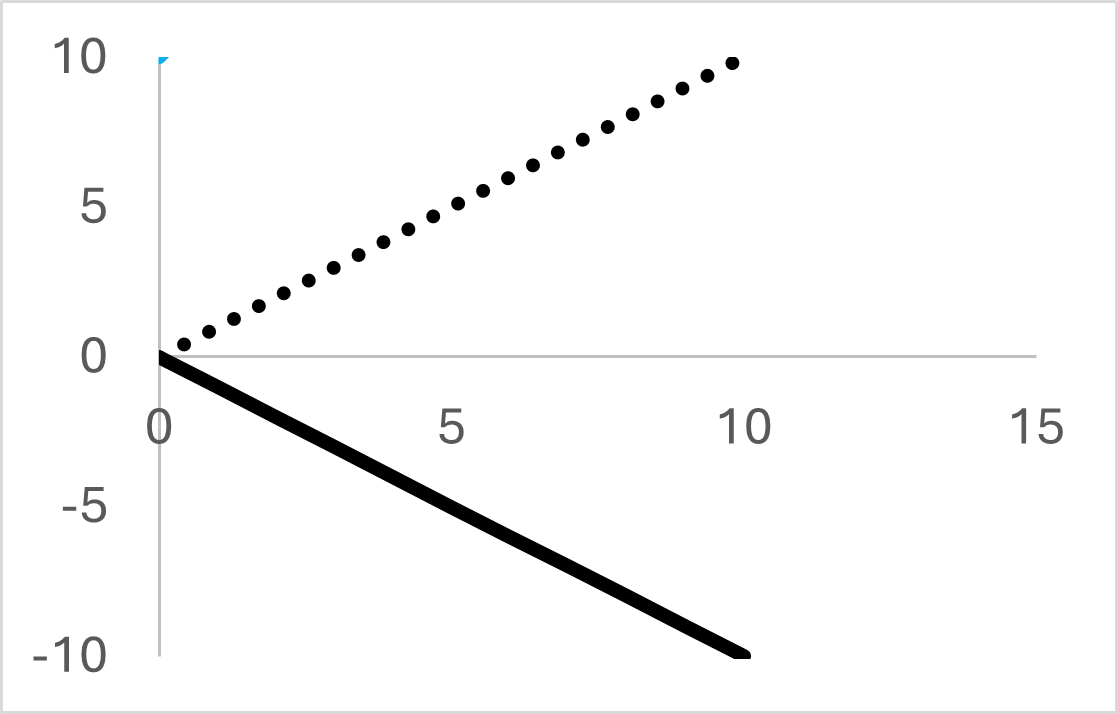
\includegraphics[width=\linewidth]{media/3a.png}
			\caption{Strong Congruence with Higher Scores on Predictor Associated with Greater Incongruence}
		\end{subfigure}
		\hfill
		\begin{subfigure}[t]{0.45\textwidth}
			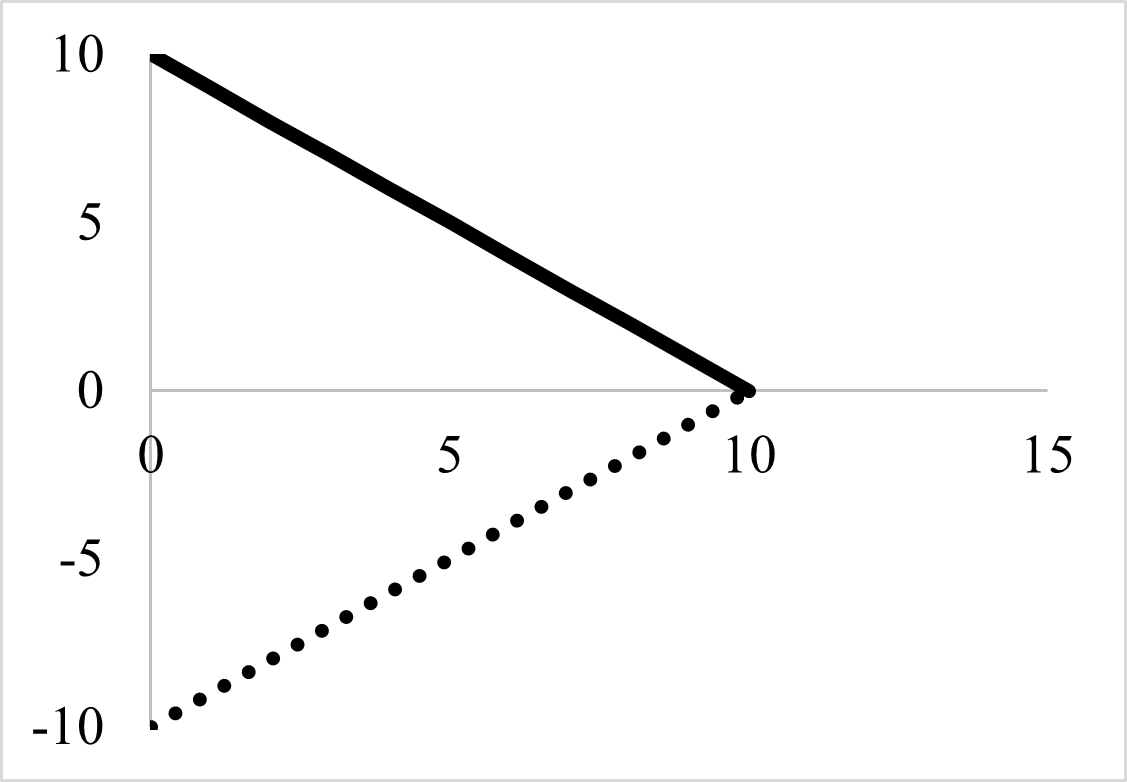
\includegraphics[width=\linewidth]{media/3b.png}
			\caption{Strong Congruence with Higher Scores on Predictor Associated with Greater Congruence}
		\end{subfigure}


		\begin{subfigure}[t]{0.45\textwidth}
			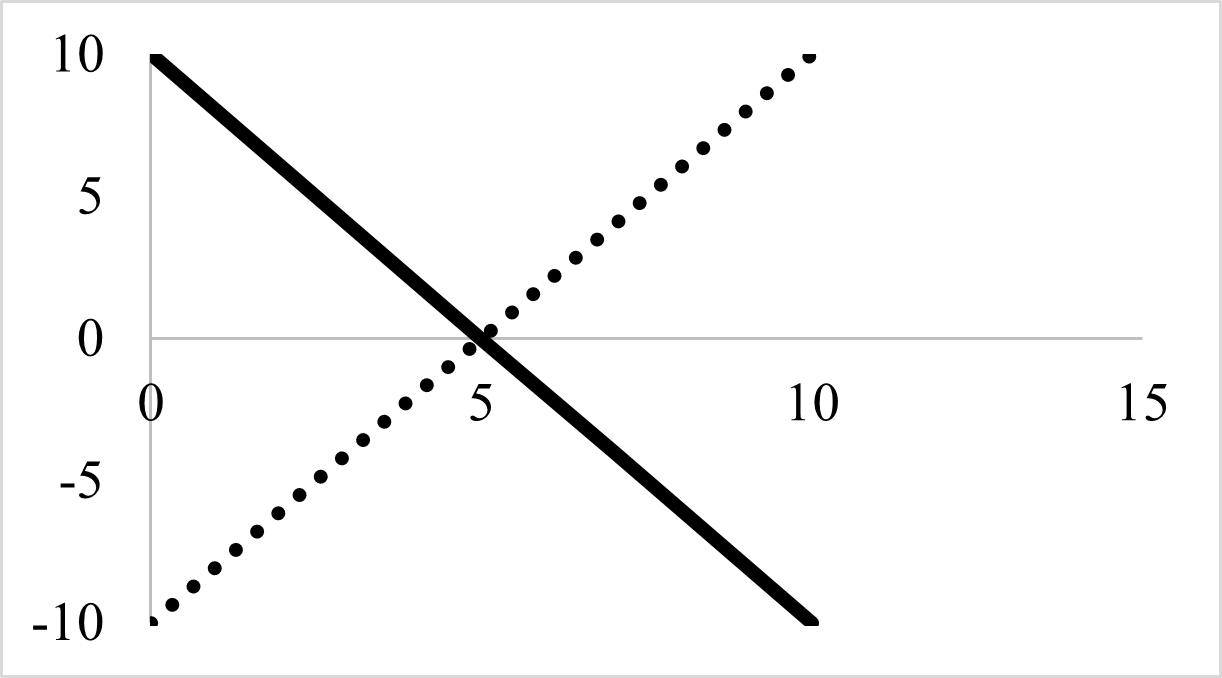
\includegraphics[width=\linewidth]{media/3c.png}
			\caption{Mixed Strong Congruence}
		\end{subfigure}
		\hfill
		\begin{subfigure}[t]{0.45\textwidth}
			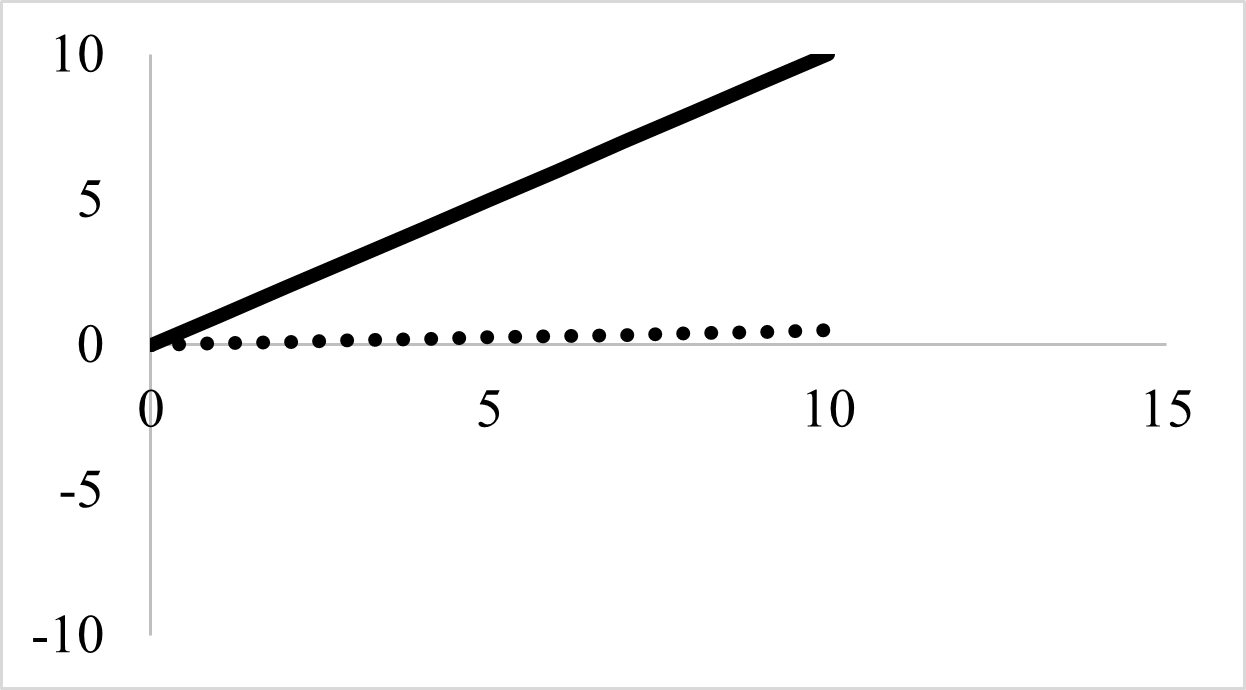
\includegraphics[width=\linewidth]{media/3d.png}
			\caption{Weak Congruence}
		\end{subfigure}


		\begin{subfigure}[t]{0.45\textwidth}
			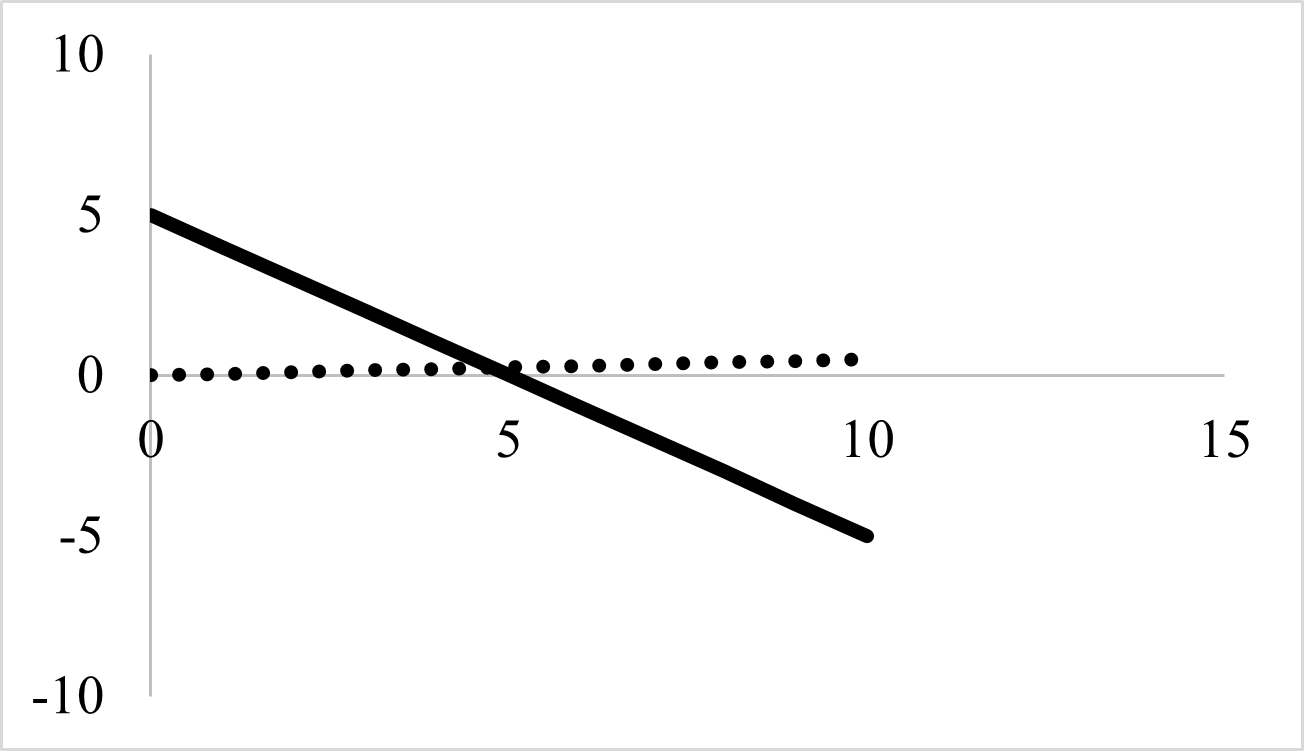
\includegraphics[width=\linewidth]{media/3e.png}
			\caption{Mixed Weak Congruence -- Negative Slope}
		\end{subfigure}
		\hfill
		\begin{subfigure}[t]{0.45\textwidth}
			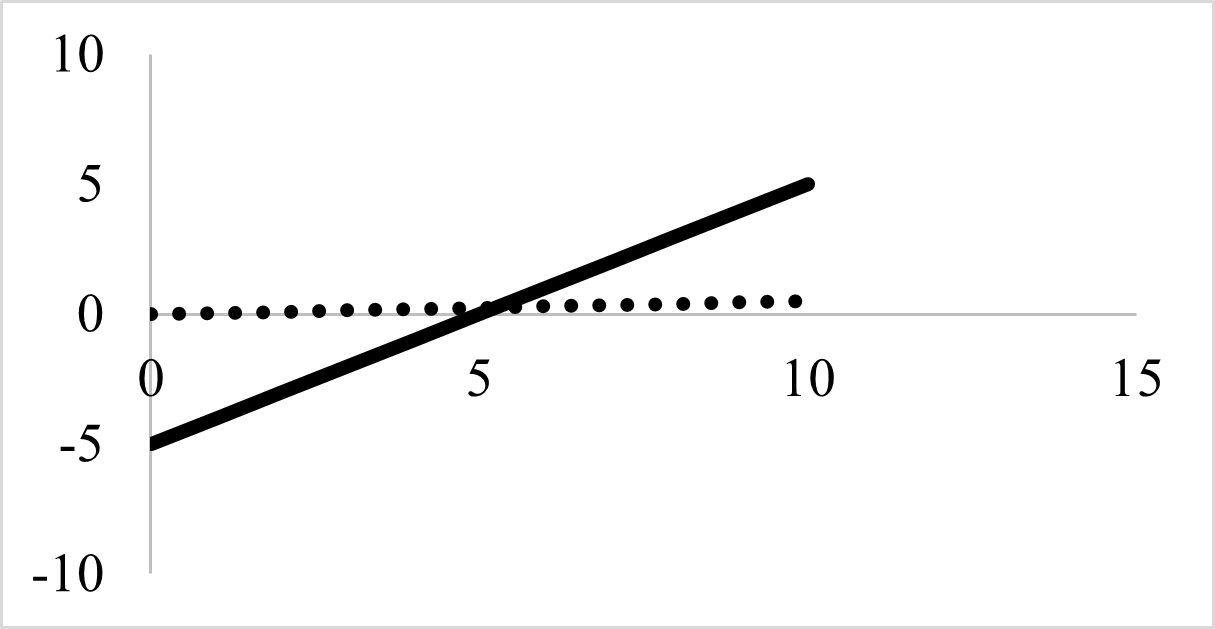
\includegraphics[width=\linewidth]{media/3f.png}
			\caption{Mixed Weak Congruence -- Positive Slope}
		\end{subfigure}


		\begin{subfigure}[t]{0.45\textwidth}
			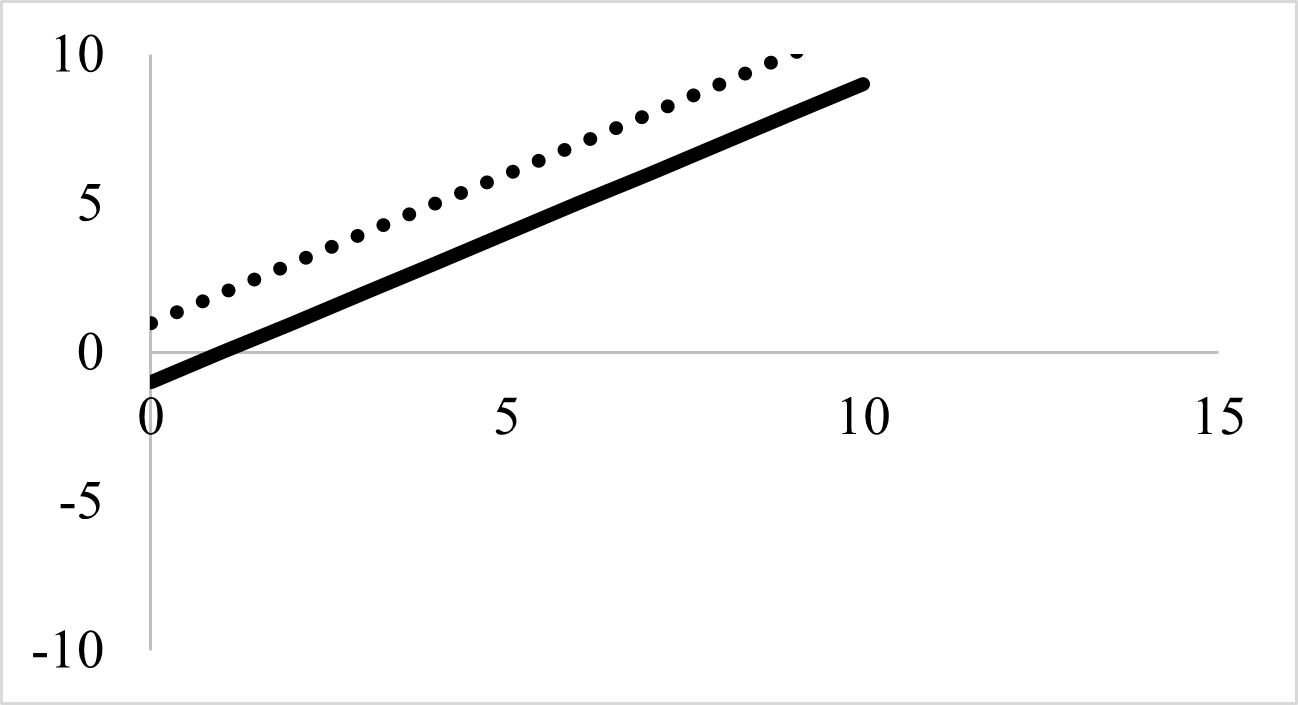
\includegraphics[width=\linewidth]{media/3g.png}
			\caption{Symmetric Linear Trend}
		\end{subfigure}
		\hfill
		\begin{subfigure}[t]{0.45\textwidth}
			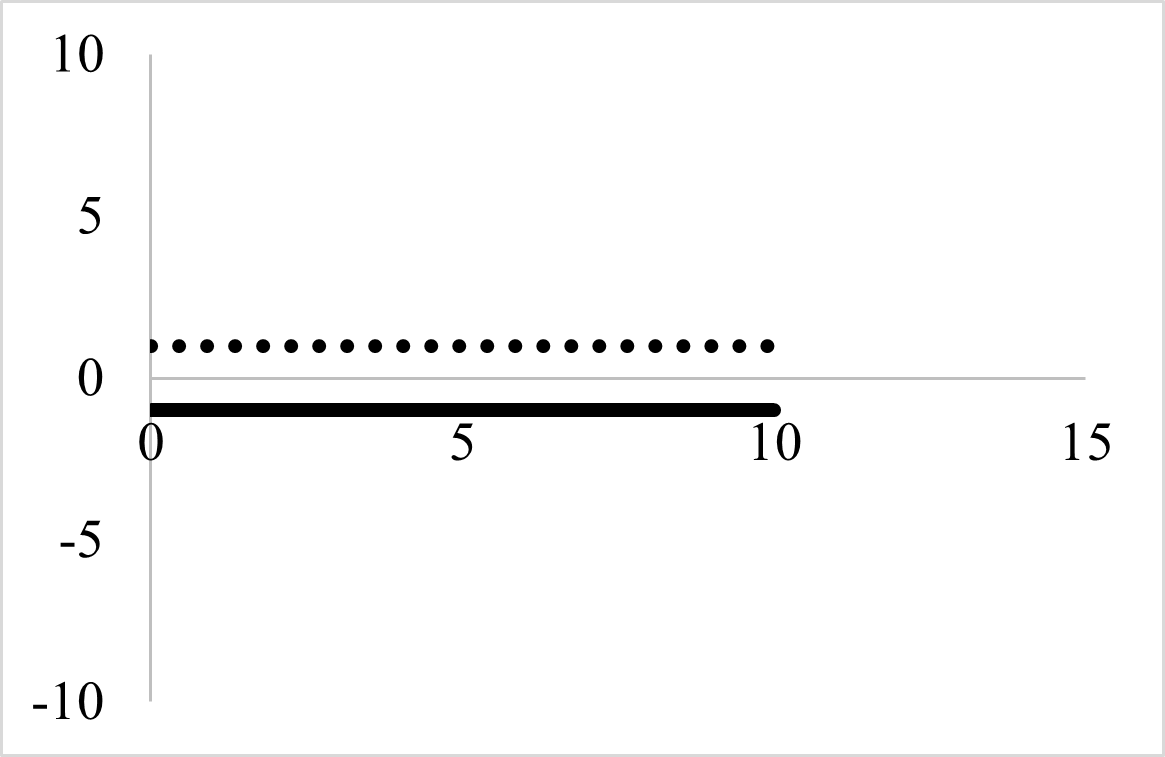
\includegraphics[width=\linewidth]{media/3h.png}
			\caption{Weak or Null Effect}
		\end{subfigure}
	\end{figure*}


	\subsection{\emph{}}



	\begin{figure}
		
\includegraphics[width=\linewidth]{media/image3.png}

		\caption{Interaction Between Defense Spending Attitudes and Being a Democrat on Affective Polarization\\\emph{Note}. Blue line represents association among Democrats, and red line represents association among Republicans.}

		\label{fig:rId60}


	\end{figure}




	\begin{figure}
		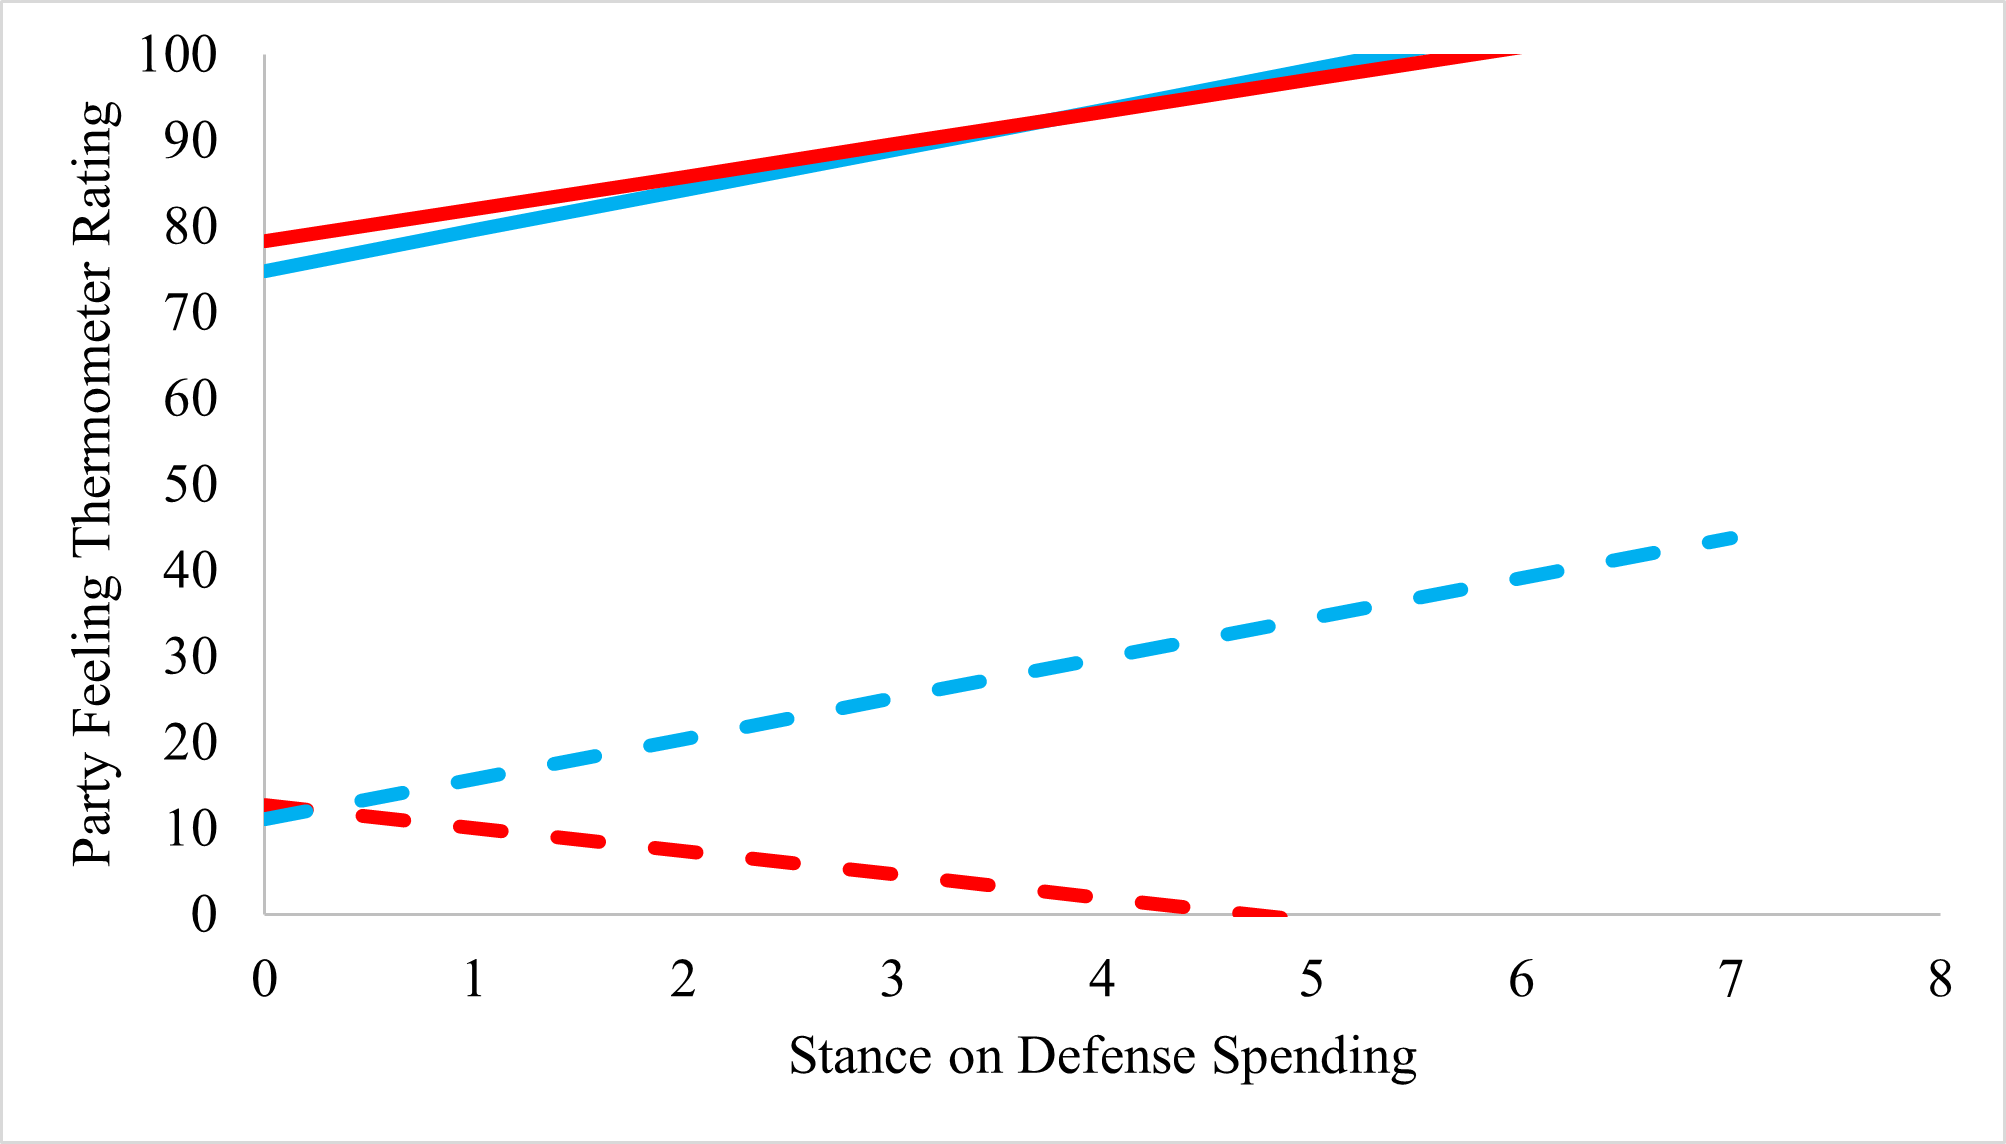
\includegraphics[width=\linewidth]{media/final.png}
		\caption{Association Between Defense Spending Attitudes and Feeling Thermometer Ratings of Each Party\\\emph{Note.} Higher scores on defense spending variable indicate more conservative stances, while lower scores indicate more liberal stances. Red lines = regression line for Republican-leaning participants; blue lines = regression line for Democrat-leaning participants; Solid lines = inparty ratings; dashed lines = outparty ratings. Figure created with parameter estimates.}


	\end{figure}



	









\end{document}